\documentclass[9pt,fleqn,ngerman,article]{memoir}

\title{Mechanik III -- Zusammenfassung}
\author{Philipe Fatio}

%% Memoir layout setup

%% NOTE: You are strongly advised not to change any of them unless you
%% know what you are doing.  These settings strongly interact in the
%% final look of the document.

% Dependencies
\usepackage{array}
\usepackage{wrapfig}
\usepackage{multicol}
\usepackage[thmmarks]{ntheorem}

\columnsep 30pt
\columnseprule \normalrulethickness

% Define the default sans serif font as the lighter computer modern bright by
% D. Knuth.
\renewcommand{\sfdefault}{cmbr}

\makeatletter

% Set the way pages are layed out (headers and page numbering)
\makepagestyle{mystyle}
\makeheadrule{mystyle}{\textwidth}{\normalrulethickness}
\makeoddhead{mystyle}{\textsc{\@title}}{}{\emph{\@author} -- \today{}}
\makeevenhead{mystyle}{\textsc{\@title}}{}{\emph{\@author} -- \today{}}
\makeoddfoot{mystyle}{}{\small -- \thepage{} --}{}
\makeevenfoot{mystyle}{}{\small -- \thepage{} --}{}
\pagestyle{mystyle}

% Use the newly defined style
\chapterstyle{VZ14}

% Redefine sectional headings to contain rules
\renewcommand{\section}{\@startsection{section}{1}{0mm}%
{-2\baselineskip}{0.8\baselineskip}%
{\hrule depth 0.2pt width\columnwidth\hrule depth1.5pt
width0.25\columnwidth\vspace*{1.2em}\Large\bfseries\sffamily}}
\makeatother

\makeatletter
\renewcommand{\subsection}{\@startsection{subsection}{1}{0mm}%
{-2\baselineskip}{0.8\baselineskip}%
{\hrule depth 0.2pt width\columnwidth\hrule depth0.75pt
width0.25\columnwidth\vspace*{1.2em}\large\bfseries\sffamily}}
\makeatother

\makeatletter
\renewcommand{\subsubsection}{\@startsection{subsubsection}{1}{0mm}%
{-2\baselineskip}{0.8\baselineskip}%
{\hrule depth 0.2pt width\columnwidth\vspace*{1.2em}\normalsize\bfseries\sffamily}}

\renewcommand*{\thesection}{\arabic{section}}

\setparaheadstyle{\normalsize\bfseries\sffamily}
\setsubparaheadstyle{\normalsize\bfseries\sffamily}

% Set captions to a more separated style for clearness
\captionnamefont{\sffamily\bfseries\footnotesize}
\captiontitlefont{\sffamily\footnotesize}
\setlength{\intextsep}{16pt}
\setlength{\belowcaptionskip}{1pt}

% Set section and TOC numbering depth to subsection
\setsecnumdepth{subsection}
\settocdepth{subsection}

% Turn off american style paragraph indentation and add some space to be
% printed when a new paragraph starts.

\setlength{\parindent}{0pt}
\addtolength{\parskip}{1pt}

\setlength{\droptitle}{-2em}
\renewcommand{\maketitlehookb}{\vspace{-1em}}
\date{}

% A bit spacier tabulars and lists
\setlength{\extrarowheight}{4pt}
\setlength{\itemsep}{10pt}
% \renewcommand{\arraystretch}{1.2}

% % This provides a frontend to set the lecture date into the header
% \newcommand{\lecturedate}[1]{\def\@lecdate{#1}}
% \makeoddhead{Ruled}{\@lecdate}{}{\normalfont\rightmark}

\makeatother

% This defines how theorems should look. Best leave as is.
\theoremstyle{plain}
\theoremseparator{:\quad}
\theoremprework{}
\theoremindent2em
\theoremheaderfont{\sffamily\bfseries}
\theorembodyfont{\normalfont}
\theoremsymbol{}

% redefine the over/underbrace to get more lightweight braces (borrowed from MnSymbols)
\makeatletter
\DeclareSymbolFont{largesymbolsA}{U}{txexa}{m}{n}
\def\re@DeclareMathSymbol#1#2#3#4{%
    \let#1=\undefined
    \DeclareMathSymbol{#1}{#2}{#3}{#4}}
\re@DeclareMathSymbol{\br@cext}{\mathord}{largesymbolsA}{"20}
\DeclareSymbolFont{extsymbols}{OMX}{txex}{m}{n}
\re@DeclareMathSymbol{\braceld}{\mathord}{extsymbols}{"7A}
\re@DeclareMathSymbol{\bracerd}{\mathord}{extsymbols}{"7B}
\re@DeclareMathSymbol{\bracelu}{\mathord}{extsymbols}{"7C}
\re@DeclareMathSymbol{\braceru}{\mathord}{extsymbols}{"7D}
\def\downbracefill{$\m@th%
   \braceld\mkern-1mu\cleaders\hbox{$\mkern-.5mu\br@cext\mkern-.5mu$}%
   \hfill\mkern-1mu%
   \braceru\bracelu%
   \mkern-1mu\cleaders\hbox{$\mkern-.5mu\br@cext\mkern-.5mu$}%
   \hfill\mkern-1mu\bracerd$}
 \def\upbracefill{$\m@th%
   \bracelu\mkern-1mu\cleaders\hbox{$\mkern-.5mu\br@cext\mkern-.5mu$}%
   \hfill\mkern-1mu%
   \bracerd\braceld%
   \mkern-1mu\cleaders\hbox{$\mkern-.5mu\br@cext\mkern-.5mu$}%
   \hfill\mkern-1mu\braceru$}
\makeatother

% index for multicols
\makeatletter
\renewenvironment{theindex}
  {\if@twocolumn
      \@restonecolfalse
   \else
      \@restonecoltrue
   \fi
   \begin{multicols*}{3}[\paragraph*{\indexname}]
   \markboth{\MakeUppercase\indexname}%
            {\MakeUppercase\indexname}%
   \thispagestyle{mystyle}
   \setlength{\parindent}{0pt}
   \setlength{\parskip}{0pt plus 0.3pt}
   \relax
   \let\item\@idxitem}%
  {\end{multicols*}\if@restonecol\onecolumn\else\clearpage\fi}
\makeatother
\usepackage[
	a4paper,
	landscape,
	left=.75cm,
	right=.75cm,
	top=.75cm,
	bottom=0.5cm,
	includeheadfoot
]{geometry}
%% See the TeXed file for more explanations

\usepackage{babel}

\usepackage[utf8]{inputenc}
\usepackage[sc]{mathpazo}
\usepackage[thmmarks]{ntheorem}
\usepackage[nice]{nicefrac}
\usepackage[load={prefixed,prefix,abbr,named,synchem,addn},per=frac,fraction=frac]{siunitx}
\usepackage{tikz}

%% Math related packages

%% The AMS-LaTeX extensions for mathematical typesetting.
\usepackage{amsmath,amssymb,amsfonts,mathrsfs}

\renewcommand{\arraystretch}{0.8}
% import content
\newcommand{\content}[1]{
	\input{content/#1.tex}
}
% Macro for units
\newcommand{\sunit}[1]{\ensuremath{ \quad \left[ \si{#1} \right] } }
\newcommand{\nicesunit}[1]{\ensuremath{ \quad \left[ \si[fraction=nicefrac]{#1} \right] } }
\newcommand{\unit}[1]{\ensuremath{ \left[ \si{#1} \right] } }
\newcommand{\niceunit}[1]{\ensuremath{ \left[ \si[fraction=nicefrac]{#1} \right] } }

%% [OPT] Multi-rowed cells in tabulars
%\usepackage{multirow}

%% [REC] Intelligent cross reference package. This allows for nice
%% combined references that include the reference and a hint to where
%% to look for it.
\usepackage{varioref}
% \labelformat{equation}{(#1)} % keine gute idee

%% [OPT] Easily changeable quotes with \enquote{Text}
% \usepackage[german=swiss]{csquotes}

%% [REC] Format dates and time depending on locale
% \usepackage{datetime}

%% [OPT] Provides a \cancel{} command to stroke through mathematics.
\usepackage{cancel}

%% [ADV] This allows for additional typesetting tools in
%% mathmode. \mathclap{} will allow you to take away the width of a
%% mathematical statement seen by LaTeX.
\usepackage{mathtools}

%% [ADV] Conditional commands
%% (note that this is included by macrosetup.tex anyway)
%\usepackage{ifthen}

%% [OPT] Manual large braces or other delimiters.
%\usepackage{bigdelim, bigstrut}

%% [REC] Alternate vector arrows. Use the command \vv{} to get scaled
%% vector arrows.
\usepackage[h]{esvect}

%% [NEED] Some extensions to tabulars and array environments.
\usepackage{array}

%% [OPT] Provides \unit[1]{N} as a means to facilitate unit
%% typesetting as well as \nicefrac{}{} command that prints a fraction
%% in text-height. Very useful for fractions inside matrices.
%\usepackage{units}

%% [NEED] Allows to rotate elements
\usepackage{rotating}

%% [OPT] LaTeX epic/eepic graphics format support.
%\usepackage{epic,eepic}

%% [OPT] Postscript support via pstricks graphics package. Very
%% diverse applications.
%\usepackage{pstricks,pst-all}

%% [?] This seems to allow us to define some additional counters.
%\usepackage{etex}

%% [ADV] XY-Pic to typeset some matrix-style graphics
%\usepackage[all]{xy}

\usepackage{booktabs}
% \usepackage{tabulary}

% \usepackage[caption=false,format=hang]{subfig}

% \usepackage[pdftex,bookmarksopen]{hyperref}

\makeatletter

\def\@pdfborder{0 0 0}%
\let\@pdfborderstyle\@empty

\makeatother

\usepackage{longtable}

\usepackage{etex}

\usepackage{fancybox}
\setlength\shadowsize{1pt}
\usepackage{empheq}

\usepackage[setpagesize=false]{hyperref}

\usepackage{multirow}
%% Custom commands =============================================================

%% Depends on this
\usepackage{ifthen}
\usepackage{rotating}
\usepackage{xy}

%% Differential d. This sets it as proper operator in roman type. With correct
%% spacing. ISO standards for mathematical typesetting says it should be printed
%% like this.
\newcommand{\diff}[1]{\operatorname{d}\ifthenelse{\equal{#1}{}}{\,}{\!#1}}

% Einheitsmatrix
\newcommand{\I}{\mathbb{I}}

%% Symbols for euler number and imaginary unit
\providecommand*{\eu}%
{\ensuremath{\mathrm{e}}}
% The imaginary unit
\providecommand*{\iu}%
{\ensuremath{\mathrm{i}}} % i can be replaced with j on preference.

%% Ortsvektor mit römischen buchstaben
\newcommand{\pVec}[1]{\vv{r_{#1}}}

%% Uncomment below what style you prefer for printing differential operators
%\DeclareMathOperator{\grad}{grad}
%\DeclareMathOperator{\rot}{rot}
%\DeclareMathOperator{\Div}{div}
\DeclareMathOperator{\grad}{\nabla\!}
\DeclareMathOperator{\rot}{\nabla\times}
\DeclareMathOperator{\Div}{\nabla\cdot}

% complex and real operators
\renewcommand{\Im}{\mathrm{Im}}
\renewcommand{\Re}{\mathrm{Re}}

%% Additional mathematical operators
\DeclareMathOperator{\tr}{tr}
\DeclareMathOperator{\id}{Id}
\DeclareMathOperator{\Kern}{Kern}
\DeclareMathOperator{\diag}{diag}
\DeclareMathOperator{\arccot}{arccot}
\DeclareMathOperator{\Adj}{Adj}
\DeclareMathOperator{\arsinh}{arsinh}
\DeclareMathOperator{\arcosh}{arcosh}
\DeclareMathOperator{\artanh}{artanh}
\DeclareMathOperator{\const}{const}
\DeclareMathOperator{\erf}{erf}
\DeclareMathOperator{\erfc}{erfc}
\newcommand{\transp}{\mathsf T}

\newcommand{\bVec}[1]{\mathbold{#1}}

%% German variants
%\DeclareMathOperator{\Kern}{Kern}
%\DeclareMathOperator{\Bild}{Bild}
%\DeclareMathOperator{\Grad}{Grad}
%% English variants
%% \ker is provided by LaTeX
\DeclareMathOperator{\im}{im}
%% \grad is provided by LaTeX

%% Special characters for number sets, e.g. real or complex numbers.
\newcommand{\C}{\mathbb{C}}
\newcommand{\K}{\mathbb{K}}
\newcommand{\N}{\mathbb{N}}
\newcommand{\Q}{\mathbb{Q}}
\newcommand{\R}{\mathbb{R}}
\newcommand{\Z}{\mathbb{Z}}
\newcommand{\X}{\mathbb{X}}

%% Fixed size delimiter examples
\newcommand{\floor}[1]{\lfloor #1 \rfloor}
\newcommand{\ceil}[1]{\lceil #1 \rceil}
\newcommand{\seq}[1]{\langle #1 \rangle}
\newcommand{\set}[1]{\{ #1 \}}
\newcommand{\abs}[1]{\lvert #1 \rvert}
\newcommand{\norm}[1]{\lVert #1 \rVert}
\newcommand{\indic}[1]{\bigl[#1\bigr]}

%% Scaling delimiter examples
\newcommand{\Floor}[1]{\left\lfloor #1 \right\rfloor}
\newcommand{\Ceil}[1]{\left\lceil #1 \right\rceil}
\newcommand{\Seq}[1]{\left\langle #1 \right\rangle}
\newcommand{\Set}[1]{\left\{ #1 \right\}}
\newcommand{\Abs}[1]{\left\lvert #1 \right\rvert}
\newcommand{\Norm}[1]{\left\lVert #1 \right\rVert}

%% Absolute and partial derrivate fractions
\newcommand{\Diff}[2]{\displaystyle\frac{\diff{#1}}{\diff{#2}}}
\newcommand{\Part}[2]{\displaystyle\frac{\partial #1}{\partial #2}}

%% Set an index and print it to the current position at the same time
\newcommand{\Index}[1]{\emph{#1}\index{#1}}

%% Displaystyle math for inline math mode
\newcommand{\ds}{\displaystyle}

%% Easy to use alias for the default matrices with round braces
\newcommand{\Mx}[1]{\ensuremath{\begin{bmatrix}#1\end{bmatrix}}}

%% Include a lecture from the lectures/ folder by date.
\newcommand{\Include}[4][\prefix]%
{\ifthenelse{\equal{#1}{+PRE% this comment prevents substitution
FIX+}}{\Include[TP]{#2}{#3}{#4}}{\lecturedate{\formatdate{#2}{#3}{20#4}}\input{lectures/#1-#4-#3-#2.tex}}}


%% A macro to typeset a commutitive diagram in the style of
%% \[\Abb[functionname]{from}{to}{fromelement}{toelement}\]
\newcommand{\Sidein}{\begin{rotate}{90}\small$\in$\end{rotate}}
\newcommand{\sidew}[1]{\rotatebox{90}{\small$#1$}}

\newcommand{\Abb}[5][]{\ensuremath{
    \begin{array}{lc}
      \ifthenelse{\equal{#1}{}}{}{#1:}\;\; &
      \begin{xy}
        \xymatrixrowsep{1em}\xymatrixcolsep{2em}%
        \xymatrix{ #2 \ar[r] \ar@{}[d]^<<<<{\hspace{0.001em} \Sidein}
          & #3  \ar@{}[d]^<<<<{\hspace{0.001em} \Sidein} \\
          #4 \ar@{|->}[r] & #5} \end{xy}
    \end{array}
  }%
}


%% Use the alternative epsilon per default and define the old one as \oldepsilon
\let\oldepsilon\epsilon

\renewcommand{\epsilon}{\ensuremath\varepsilon}

%% Also set the alternate phi as default.
\renewcommand{\phi}{\ensuremath{\varphi}}

%% Table centering header
\newcommand{\ctabletitle}[2]{\multicolumn{#1}{c}{\bfseries#2}}

%% emphasized equation
\newcommand{\emphequation}[2]{
	\begin{empheq}[box=\shadowbox*]{#1}
		#2
	\end{empheq}%
}

% renew \abs so the bars are adjusted to the height of the content
\renewcommand{\abs}[1]{\ensuremath{\left|#1\right|}}

% conditional equation with large left curly brace
\newcommand{\conditional}[1]{
\left\{\begin{array}{@{}l@{\quad}l}
	#1
\end{array}\right.
}

% parentheses
\newcommand{\parens}[1]{\ensuremath{\left(#1\right)}}

% 1/2 fractions
\newcommand{\half}{\ensuremath{\frac{1}{2}}}
\newcommand{\nicehalf}{\ensuremath{\nicefrac{1}{2}}}

%% tighter itemize
\newenvironment{tightitemize}
	{
	\begin{itemize}
	\setlength{\itemsep}{2pt}
	\setlength{\parskip}{0pt}
	\setlength{\parsep}{0pt}
	}
	{\end{itemize}}

%% tighter enumerate
\newenvironment{tightenumerate}
	{
	\begin{enumerate}
	\setlength{\itemsep}{2pt}
	\setlength{\parskip}{0pt}
	\setlength{\parsep}{0pt}
	}
	{\end{enumerate}}

%% Handy Envs
\newenvironment{definition}
	{\textsc{Definition:}\ }

\newenvironment{theorem}
	{\textsc{Theorem:}\ }

\newenvironment{notation}
	{\textsc{Notation:}\ }

\newenvironment{beispiel}
	{\textsc{Beispiel:}\ }

\newenvironment{satz}
	{\textsc{Satz:}\ }

\newenvironment{bedingung}
	{\textsc{Bedingung:}\ }

\newenvironment{achtung}
	{\textsc{Achtung:}\ }

\newenvironment{bedingungen}
	{
	\textsc{Bedingungen:}
	\vspace{-2ex}
	\begin{tightitemize}
	}
	{\end{tightitemize}}

\newenvironment{bemerkung}
	{\textsc{Bemerkung:}\ }
	
\newenvironment{bemerkungen}
	{
	\textsc{Bemerkungen:}
	
	\begin{tightitemize}
	}
	{\end{tightitemize}}

\newenvironment{folgerung}
	{\textsc{Folgerung:}\ }

\newenvironment{algo}
	{\textsc{Algorithmus:}\ }

\newenvironment{folgerungen}
	{
	\textsc{Folgerungen:}
	
	\begin{tightitemize}
	}
	{\end{tightitemize}}

\newenvironment{regeln}
	{
	\textsc{Regeln:}
	
	\begin{tightitemize}
	}
	{\end{tightitemize}}


\usetikzlibrary{decorations}
\usetikzlibrary{arrows}

\usetikzlibrary{%
    decorations.pathreplacing,%
    decorations.pathmorphing%
}

\usetikzlibrary{calc}

\makeatletter
\pgfarrowsdeclare{smo}{smo}
{
  \pgfarrowsleftextend{+-.5\pgflinewidth}
  \pgfutil@tempdima=0.2pt%
  \advance\pgfutil@tempdima by.2\pgflinewidth%
  \pgfutil@tempdimb=9\pgfutil@tempdima\advance\pgfutil@tempdimb by.5\pgflinewidth
  \pgfarrowsrightextend{+\pgfutil@tempdimb}
}
{
  \pgfutil@tempdima=0.2pt%
  \advance\pgfutil@tempdima by.2\pgflinewidth%
  \pgfsetdash{}{+0pt}
  \pgfpathcircle{\pgfqpoint{4.5\pgfutil@tempdima}{0bp}}{4.5\pgfutil@tempdima}
  \pgfusepathqstroke
}

\makeatother

\tikzset{interface/.style={
        % The border decoration is a path replacing decorator. 
        % For the interface style we want to draw the original path.
        % The postaction option is therefore used to ensure that the
        % border decoration is drawn *after* the original path.
        postaction={draw,decorate,decoration={border,angle=-45,
                    amplitude=0.3cm,segment length=2mm}}},
	feder/.style={
		decorate,decoration={coil,post length=.15cm, pre length=.15cm},segment length=4pt
	}
}

\newcommand{\kreisel}[3]{
\def\ellAdj{.43}
\path[draw,fill=gray!20] (#2/2/#3,0) ellipse (\ellAdj*#1*#3 and #1) ;
\path[draw,shade,bottom color=gray!40,top color=gray!30,middle color=gray!5] (#2/2/#3, #1) -- ++ (-#2/#3,0) arc (90:270:\ellAdj*#1*#3 and #1) -- ++ (#2/#3,0) arc (270:90:\ellAdj*#1*#3 and #1);
}

\newcommand{\measurement}[4][]{%
\def\ruleInset{3pt}

\draw #2 -- ++ #4 coordinate(tmpa) ++ ($(0,0)!1!90:#4$) coordinate(tmpb);
\draw #3 -- ($(tmpa)!#3!(tmpb)$) coordinate(tmpc);

\draw[<->] (tmpa) ++ ($(0,0)!-\ruleInset!#4$) -- ($(tmpc) + (0,0)!-\ruleInset!#4$) node[midway,sloped,below]{#1};
}


% \setlength{\parindent}{5pt}

\renewcommand{\vec}{\ensuremath{\mathbold}}
% vector in another system
\newcommand{\vecin}[2]{\ensuremath{{}_{#2}\vec{#1}}}
\newcommand{\mtrx}{\ensuremath{\mathbold}}
% transformation matrix
\newcommand{\trafo}[2]{\ensuremath{\mtrx{#1}_{#2}}}
% Winkelgeschwindigkeit zwischen Systemen im System:
\newcommand{\momegain}[2]{\ensuremath{{}_{#2}\trafo{\widetilde \omega}{#1}}} % matrix
\newcommand{\omegain}[2]{\ensuremath{{}_{#2}\trafo{\omega}{#1}}}
\newcommand{\highdot}{\ensuremath{\dot{\!\!\phantom{I}}}}

% nicer tables
%\usepackage{booktabs}

\hypersetup{
    bookmarks=true,         % show bookmarks bar?
    unicode=true,          % non-Latin characters in Acrobat’s bookmarks
%    pdftoolbar=true,        % show Acrobat’s toolbar?
%    pdfmenubar=true,        % show Acrobat’s menu?
    pdffitwindow=true,     % window fit to page when opened
    pdfstartview={FitH},    % fits the width of the page to the window
    pdftitle={Mechanik III -- Zusammenfassung},    % title
    pdfauthor={Philipe Fatio},     % author
%    pdfsubject={Zusammenfassung},   % subject of the document
%    pdfcreator={Creator},   % creator of the document
%    pdfproducer={Producer}, % producer of the document
%    pdfkeywords={keywords}, % list of keywords
    pdfnewwindow=true,      % links in new window
    colorlinks=true,       % false: boxed links; true: colored links
    linkcolor=black,          % color of internal links
    citecolor=black,        % color of links to bibliography
    filecolor=black,      % color of file links
    urlcolor=black           % color of external links
}

\begin{document}
	\frontmatter
	\thispagestyle{empty}
	\begin{center}
		\begin{minipage}{0.3\linewidth}
			\vskip 1cm

			\begin{flushleft}
				\HUGE\textsc{Mechanik III}
			\end{flushleft}
			\vspace{-9.5mm}
			\begin{flushright}
				\today
			\end{flushright}
			\vspace{-5mm}
			\hbox to \hsize{\hfill
			\vrule height 1pt width\hsize
			\hfill}%
			\vspace{-3.75mm}
			\begin{flushleft}
				\Large\textsc{Zusammenfassung}
			\end{flushleft}
			\vspace{-9.55mm}
			\begin{flushright}
				\emph{Philipe Fatio}
			\end{flushright}
			\vspace{1cm}

			\vskip 4cm
			\tableofcontents*
		\end{minipage}
	\end{center}
	\thispagestyle{empty}
	\clearpage
	\mainmatter
	\begin{multicols*}{3}
		\section{Grundlegende Konzepte} % (fold)
			\subsection{Impuls \& Drall} % (fold)
				
				\paragraph{Impuls:} % (fold)
					$
						\vec{p} := m \cdot \vec{r}_{OS} \sunit{\kilogram\metre\per\second} = \unit{\newton\second}
					$
				% paragraph: Impuls: (end)
				\paragraph{Drall:} % (fold)
					$
						L_O := \underbrace{ m \cdot \vec{r}_{OS} \diamond \dot{\vec{r}}_{OS} }_{\mathclap{\text{Impulsmoment}}} + \underbrace{ \theta_S \dot{\varphi} }_{\mathclap{\text{Spin}}} \sunit{\newton\second\metre}
					$ \\
					wobei $\theta_S$ Massenträgheitsmoment bez. $S$ ist.
					
					Drall ist additiv bei gemeinsamen Bezugspunkt.
				% paragraph: Drall: (end)
			% subsection: Impuls \& Drall (end)
			
			\subsection{Massenträgheitsmoment} % (fold)
				Massenträgheitsmoment eines Körpers $B$
				\begin{description}
					\item[bezüglich Punkt $P$:]
					\begin{align*}
						\theta_P &= \int_B (x^2 + y^2) \diff m \\
						&= \iiint_B (x^2 + y^2) \rho(x,y) \diff x \diff y \diff z
					\end{align*}
					
					\item[bezüglich Schwerpunkt $S$:]
					Mit Hilfe eines Koordinatensystems mit $O$ in $S$:
					\[
						\theta_S = \int_B (\widetilde{x}^2 + \widetilde{y}^2) \diff m
					\]
					
					\item[Additivität:]
					Mehrere Trägheitsmomente bezüglich eines Punktes verhalten sich additiv.
				\end{description}
				
				\subsubsection{Satz von Steiner} % (fold)
					\[
						\theta_P = \theta_S + m \cdot a^2
					\]
					wobei $a$ der Abstand zwischen $P$ und $S$ ist.
				% subsubsection: Satz von Steiner (end)
				
				\subsection{Allgemeine Massenträgheitsmomente} % (fold)
				
					$\rho = \text{const}.$
					
					\begin{center}
						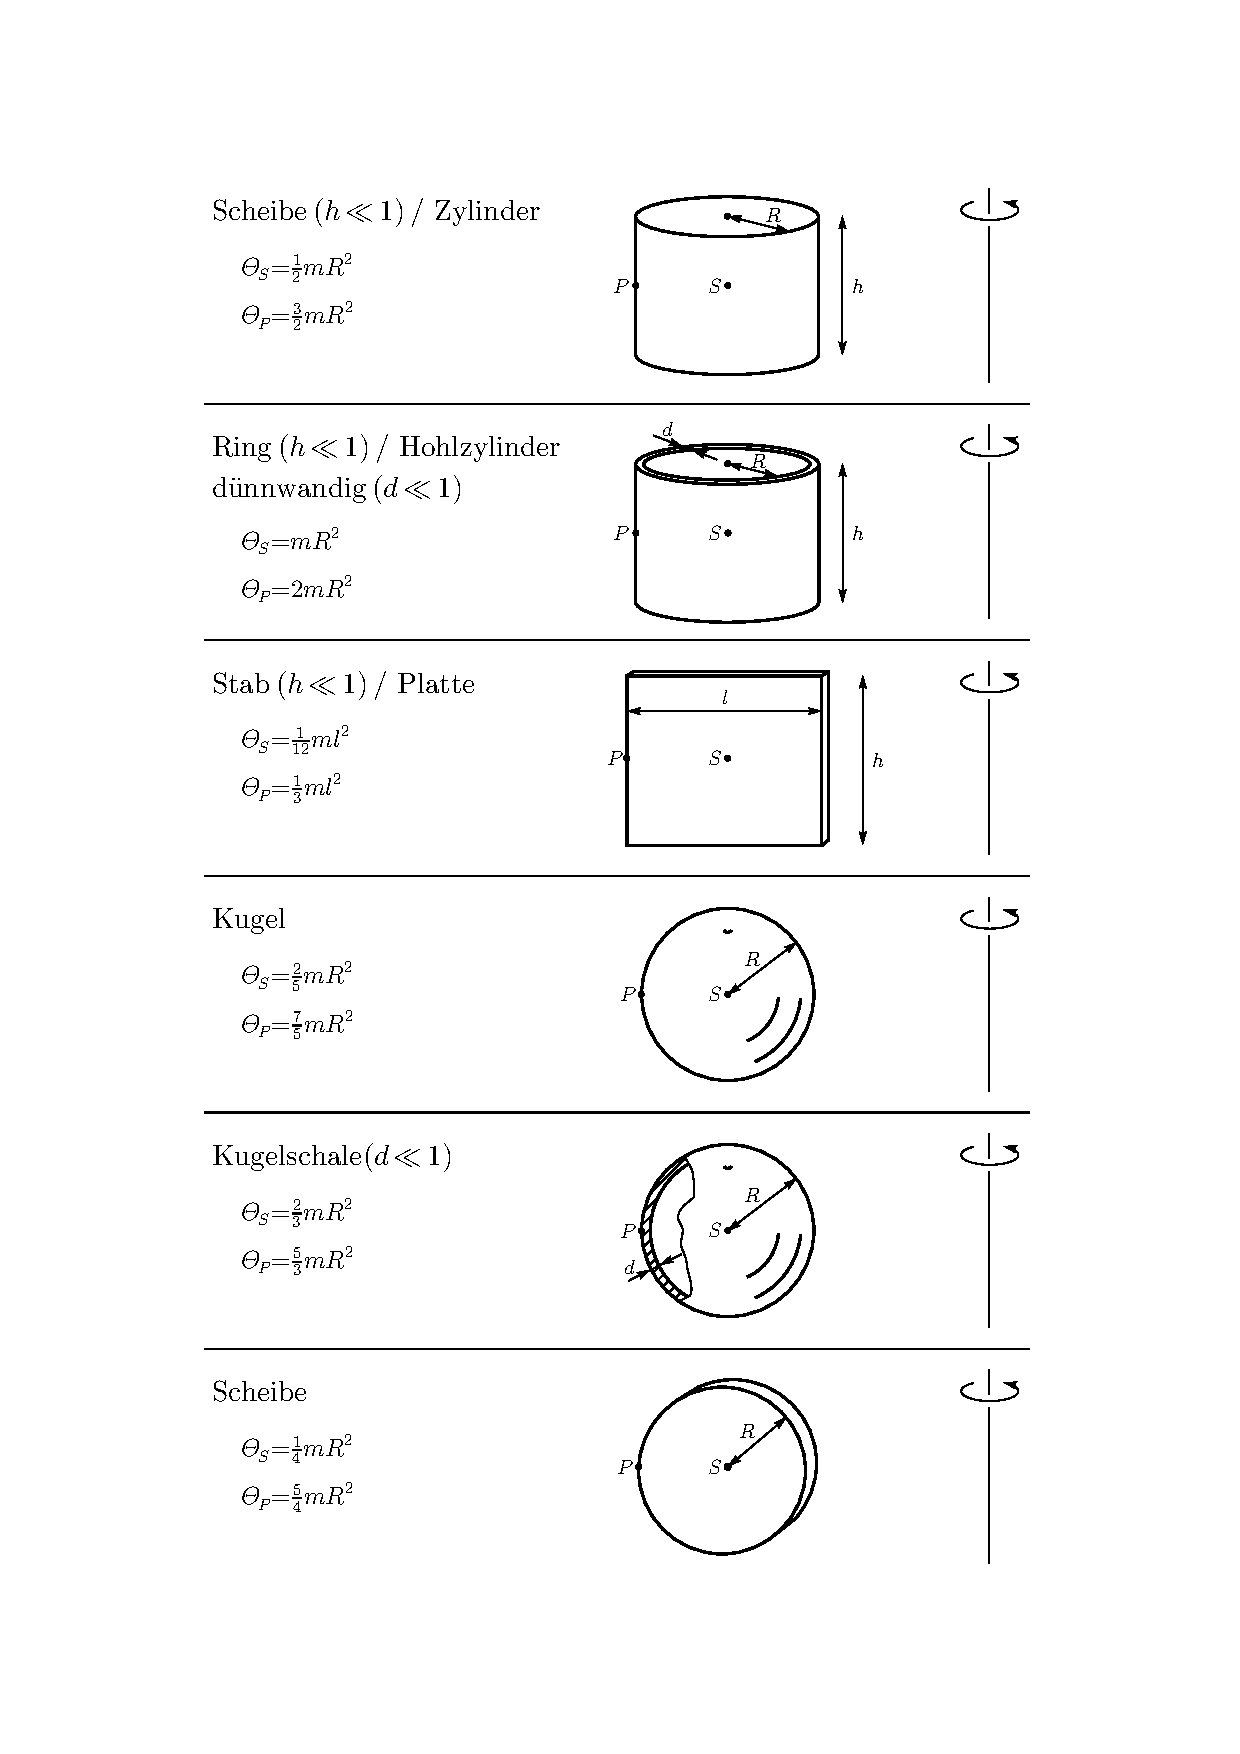
\includegraphics[width=\columnwidth]{grafiken/massentraegheitsmomente}
					\end{center}
					
				% subsection: Allgemeine Massenträgheitsmomente (end)
			% subsection: Massenträgheitsmoment (end)
			\subsection{Impuls- \& Drallsatz} % (fold)
				\paragraph{Impulssatz} % (fold)
					
					\emphequation{equation*}{
						\dot{\vec p} = m \cdot \ddot{\vec{r}}_{OS} = \sum_i \vec{F}_{P_i} \sunit{N}
					}
					
				% paragraph: Impulssatz (end)
				
				\paragraph{Drallsatz} % (fold)
					
					\emphequation{equation*}{
						\dot{\vec L}_S = \theta_S \ddot{\varphi} = \vec{r}_{SP} \diamond \vec{F}_P + \mtrx{M} \sunit{\newton\metre}
					}
					
				% paragraph: Drallsatz (end)
				
				Greifen keine äusseren Kräfte und/oder Momente an einem Starrkörper an, bleiben Impuls und Drall und somit auch $\dot{\vec{r}}_{OS}$ und $\dot{\varphi}$ konstant.
			% subsection: Impuls- \& Drallsatz (end)
			
			\subsection{Kraftgesetze äusserer Kräfte} % (fold)
				\begin{center}
					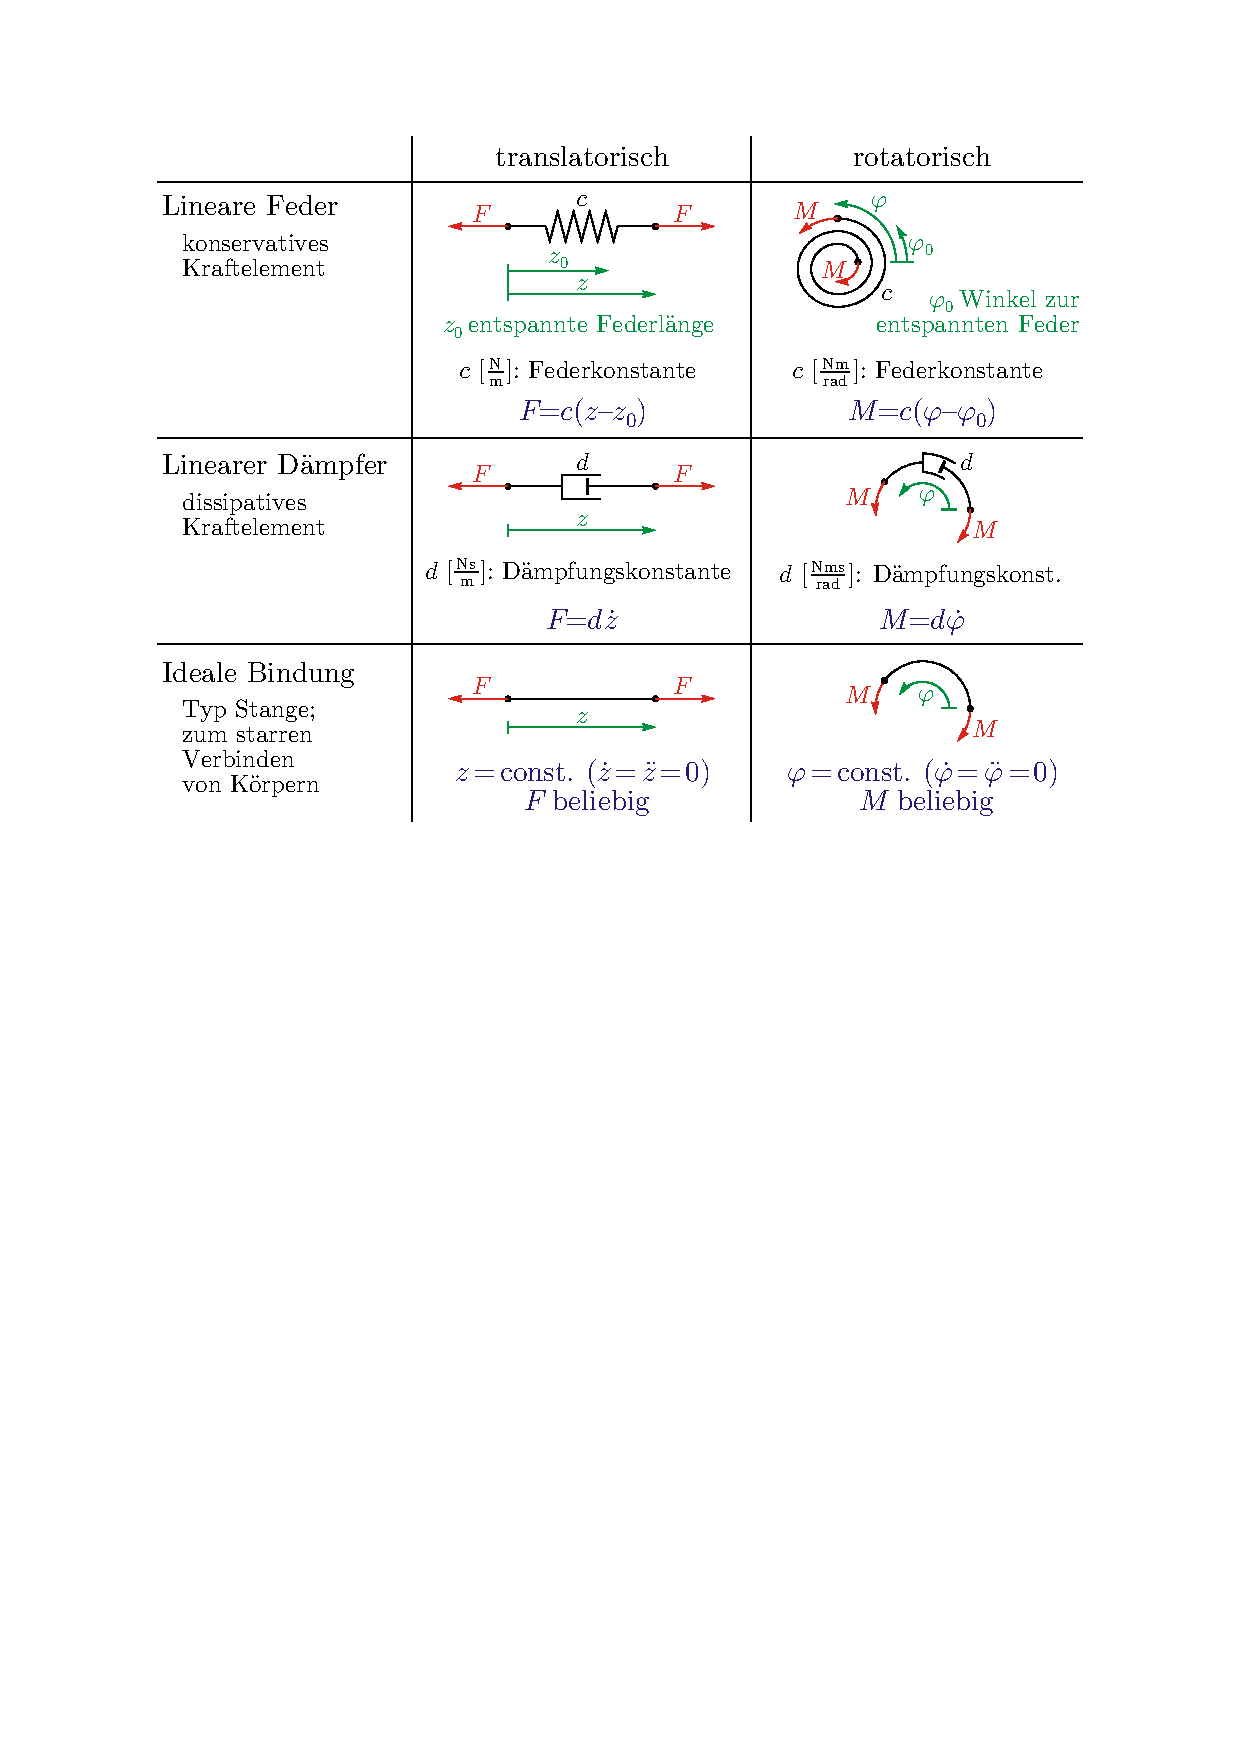
\includegraphics[width=\columnwidth]{grafiken/aeussere_kraefte}
				\end{center}
				
			% subsection: Kraftgesetze äusserer Kräfte (end)
			
			\subsection{Energie} % (fold)
				
				\subsubsection{Kinetische Energie} % (fold)
					\begin{align*}
						T &= \frac{1}{2} m \cdot \langle \dot{\vec{r}}_{OS}, \dot{\vec{r}}_{OS} \rangle + \frac{1}{2} \theta_S \dot{\varphi}^2 \sunit{\newton\metre} = \unit{\joule}\\
						&= \underbrace{\frac{1}{2} m \cdot (\dot{x}^2 + \dot{y}^2)}_{\mathclap{\text{Translationsanteil}}} + \overbrace{\frac{1}{2} \theta_S \dot{\varphi}^2}^{\mathclap{\text{Rotationsanteil}}}
					\end{align*}
				% subsubsection: Kinetische Energie (end)
				
				\subsubsection{Potentielle Energie} % (fold)
					\paragraph{Feder:} % (fold)
						\[
							V = \frac{1}{2} c \cdot (z - z_0)^2 \qquad V = \frac{1}{2} c \cdot (\varphi - \varphi_0)^2
						\]
					% paragraph: Feder (end)
					
					\paragraph{Körper im Gravitationsfeld:} % (fold)
						\[
							V = mgz
						\]
					% paragraph: Körper im Gravitationsfeld: (end)
				% subsubsection: Potentielle Energie (end)
				
				\subsubsection{Additivität} % (fold)
					Kinetische und potentielle Energien sind additiv auch wenn sie von unterschiedlichen Typen sind.
					
					\[
						T_{\text{ges}} = \sum_{i=1} T_i
						 \qquad V_{\text{ges}} = \sum_{i=1} V_i
					\]
				% subsubsection: Additivität (end)
				
				\subsubsection{Konservative Systeme} % (fold)
					Ein autonomes System aus Starrkörpern heisst \emph{konservativ}, falls alle an den einzelnen Starrkörpern angreifenden äusseren Kräfte \emph{Potentialkräfte} sind.
					
					Es gilt die Energieerhaltung:
					\[
						T_{\text{ges}} + V_{\text{ges}} = \text{const}.
					\]
					
					Systeme mit dissipativen Elementen (z.B.~Dämpfer) sind \emph{keine} konservative Systeme, da Energie verloren geht.
				% subsubsection: Konservative Systeme (end)
				
			% subsection: Energie (end)
			
			\subsection{Vorgehen bei Aufgaben} % (fold)
				\begin{enumerate}
					\item System freischneiden
					\item Koordinatensystem einführen
					\item Schwerkraft berechnen
					\item Impuls- und Drallsätze aufstellen
					\item kinematische Relationen aufstellen
					\item unbekannte Bindungskräfte eliminieren
					\item Gewichtskräfte berechnen
				\end{enumerate}
			% subsection: Vorgehen bei Aufgaben (end)
		% section: Grundlegende Konzepte (end)
		\section{Lineare Schwingungen mit einem Freiheitsgrad} % (fold)
			\paragraph{Kraftanregung} % (fold)
				\[
					m \ddot{y} + d \dot{y} + c y = F(t)
				\]
			% paragraph: Kraftanregung (end)
			\paragraph{Weganregung} % (fold)
				\[
					m \ddot{y} + d \dot{y} + c y = -m \ddot{e}(t)
				\]
				
				Lassen sich durch $F := -m \ddot{e}$ ineinander überführen.
			% paragraph: Weganregung (end)
			
			\paragraph{Matrixform} % (fold)
				\[
					\begin{array}{c@{\ =\ }c@{\cdot}c@{+}c}
					\begin{bmatrix}
						\dot{y} \\
						\ddot{y}
					\end{bmatrix}
					&
					\begin{bmatrix}
						0 & 1 \\
						-\frac{c}{m} & -\frac{d}{m}
					\end{bmatrix}
					&
					\begin{bmatrix}
						y \\
						\dot{y}
					\end{bmatrix}
					&
					\begin{bmatrix}
						0 \\
						\frac{F(t)}{m}
					\end{bmatrix}
					\\ [10pt]
					\dot{\vec{x}} & \mtrx{A} & \vec{x} & \vec{b}
					\end{array}
				\]
			% paragraph: Matrixform (end)
			\subsection{Darstellungsformen} % (fold)
				\begin{description}
					\item[Dämpfungswert:] $\delta := \frac{d}{2m} \nicesunit{\per\second}$
					\item[Eigenfrequenz:] $\omega_0 = \sqrt{\frac{c}{m}} \nicesunit{\per\second}$
				\end{description}
				
				\begin{empheq}[box=\shadowbox*]{equation*}
					\ddot{y} + 2 \delta \dot{y} + \omega_0^2 y = \frac{F(t)}{m}
				\end{empheq}
			
				Zeitunabhängig mit $\tau(t) = \omega_0 t$:
				\begin{empheq}[box=\shadowbox*]{equation*}
					\omega_0^2 y'' + 2 \delta \omega_0 y' + \omega_0^2 y = \frac{1}{m}F\left(\frac{\tau}{\omega_0}\right)
				\end{empheq}
			
				Dimensionslos mit:
				\begin{description}
					\item[Lehr'sche Dämpfung:] $D := \frac{\delta}{\omega_0} = \frac{1}{2} d \sqrt{\frac{1}{mc}} \sunit{1}$
					\item[normierte Erregerfkt:] $f(\tau) := \frac{1}{m \omega_0^2} F\left( \frac{\tau}{\omega_0} \right) \sunit{1}$
				\end{description}
				\begin{empheq}[box=\shadowbox*]{equation*}
					y'' + 2Dy' + y = f(\tau)
				\end{empheq}
			% subsection: Darstellungsformen (end)
			
			\subsection{Eigenwerte} % (fold)
				\begin{align*}
					\lambda_{1,2} &= \frac{1}{2m}\left( -d \pm \sqrt{d^2 - 4mc} \right) \\
					              &= -\frac{d}{2m} \pm \sqrt{ \left( \frac{d}{2m} \right)^2 - \frac{m}{c} } \\
					\lambda_{1,2} &= -\delta \pm \sqrt{\delta^2 - \omega_0^2} \\
					              &= \omega_0 \left( - \frac{\delta}{\omega_0} \pm \sqrt{ \left( \frac{\delta}{\omega_0} \right)^2 - 1} \right) \\
					\lambda_{1,2} &= \omega_0 \left( -D \pm \sqrt{D^2 -1} \right)
				\end{align*}
			% subsection: Eigenwerte (end)
			
			\subsection{Dämpfung} % (fold)
				\label{subsec:daempfung}
				\subsubsection{Ungedämpfte Schwingung $(D = 0)$} % (fold)
					\begin{empheq}[box=\shadowbox*]{equation*}
						\lambda_{1,2} = \pm \iu \omega_0 = \pm \iu \sqrt{\frac{c}{m}}
					\end{empheq}
					
					\[
						y_h = A \sin (\omega_0 t + \varphi) \qquad
						\dot{y}_h = \omega_0 A \cos (\omega_0 t + \varphi)
					\]
					
					\begin{description}
						\item[Frequenz:] $f_0 := \frac{\omega_0}{2\pi} \sunit{\hertz}$
						\item[Periode:] $T_0 := \frac{1}{f_0} = \frac{2\pi}{\omega_0} \sunit{s}$
					\end{description}
					
					\begin{center}
						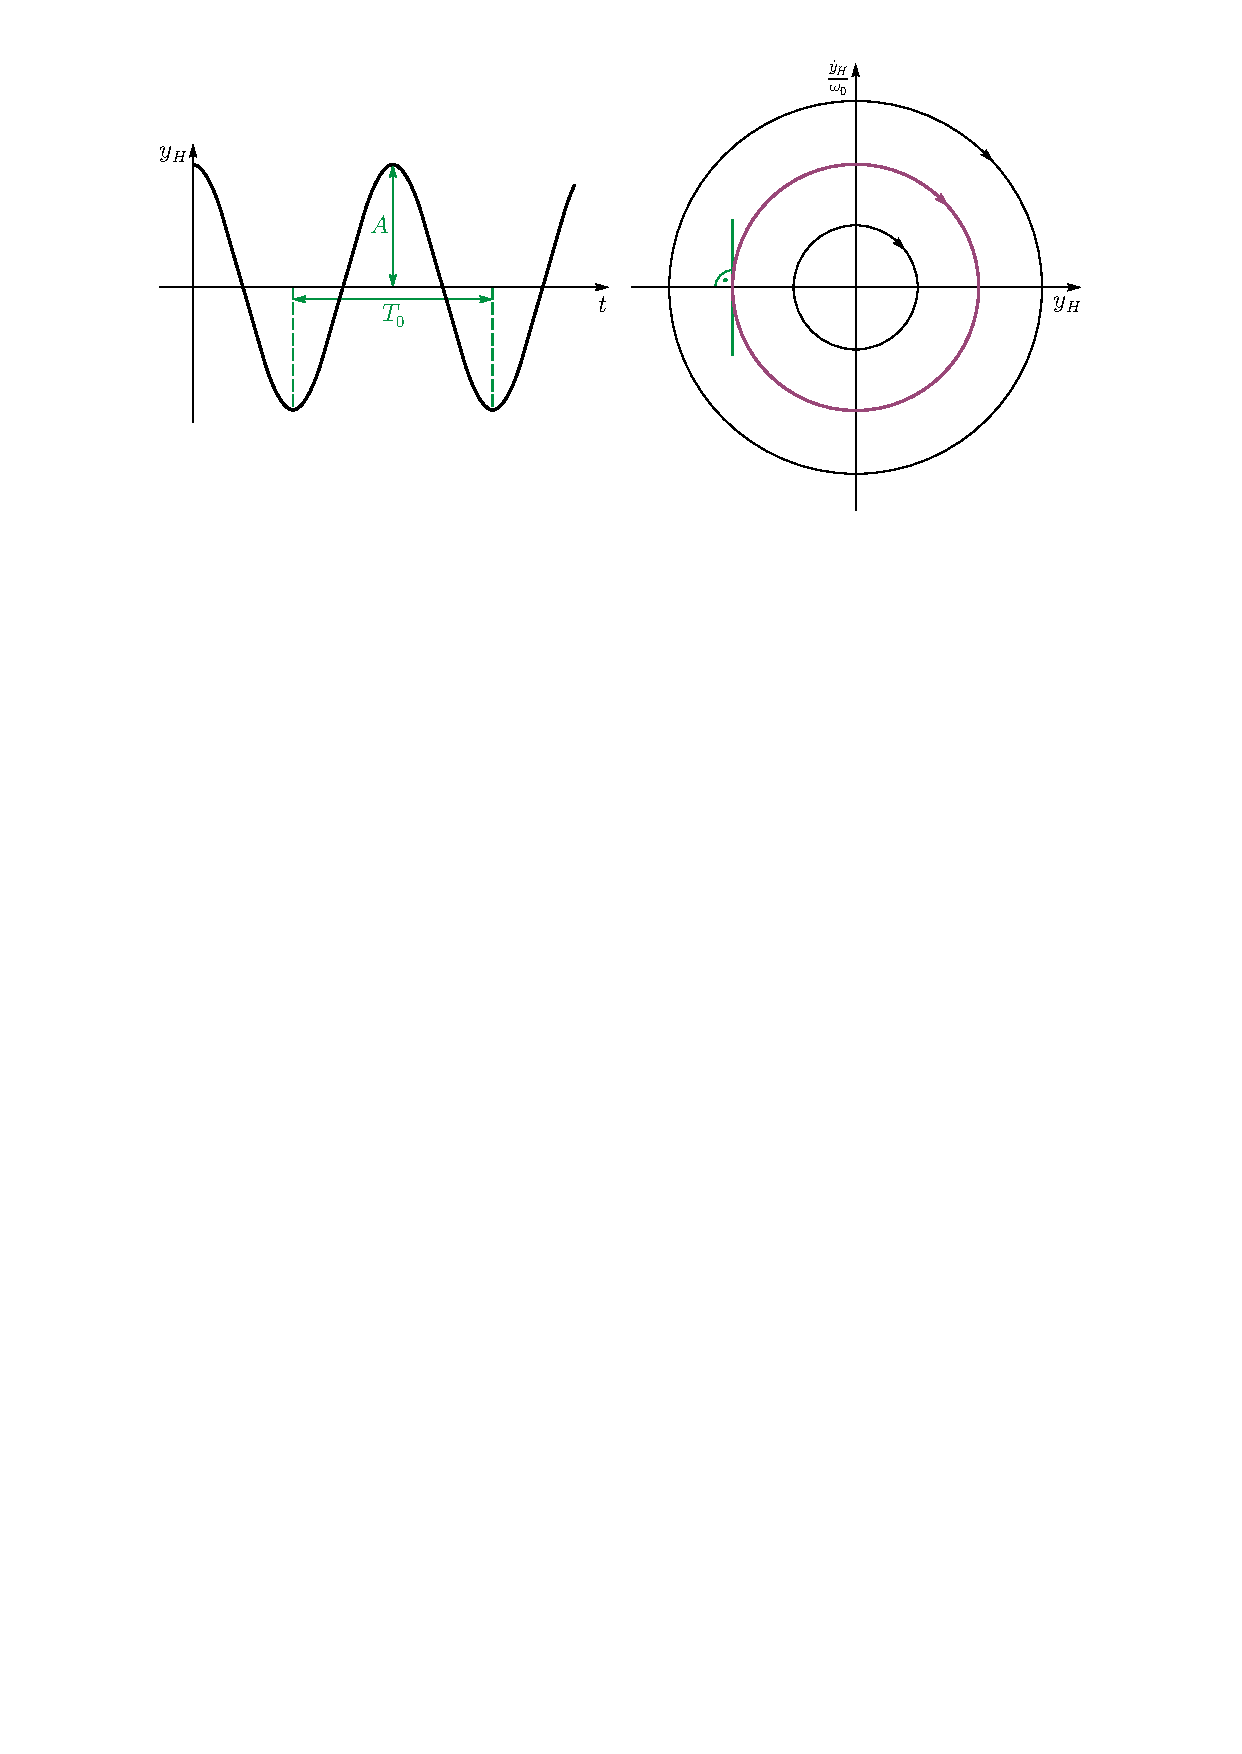
\includegraphics[width=\columnwidth]{grafiken/daempfung_d_0}
					\end{center}
					
				% subsubsection: Ungedämpfte Schwingung (D=0) (end)
				
				\subsubsection{Unterkritisch gedämpfte Schwingung $(D \in (0,1))$} % (fold)
				
					\begin{empheq}[box=\shadowbox*]{equation*}
						\lambda_{1,2} = - \delta \pm \iu \omega
					\end{empheq}
					\emph{\textbf{Achtung:}}
					\[
						\omega^2 := \omega_0^2 - \delta^2 = \omega_0^2 (1 - D^2) \qquad \omega \in (0, \omega_0)
					\]
					
					\[
						y_h = e^{-\delta t} \left( A_1 e^{\iu \omega t} + A_2 e^{-\iu \omega t} \right)
						\qquad
						\dot{y}_h = A e^{-\delta t} \cos (\omega t + \varphi)
					\]
					
					\begin{description}
						\item[Pseudofrequenz:] $f := \frac{\omega}{2\pi}$
						\item[Pseudoperiode:] $T := \frac{1}{f} = \frac{2\pi}{\omega}$
					\end{description}
					
					\begin{center}
						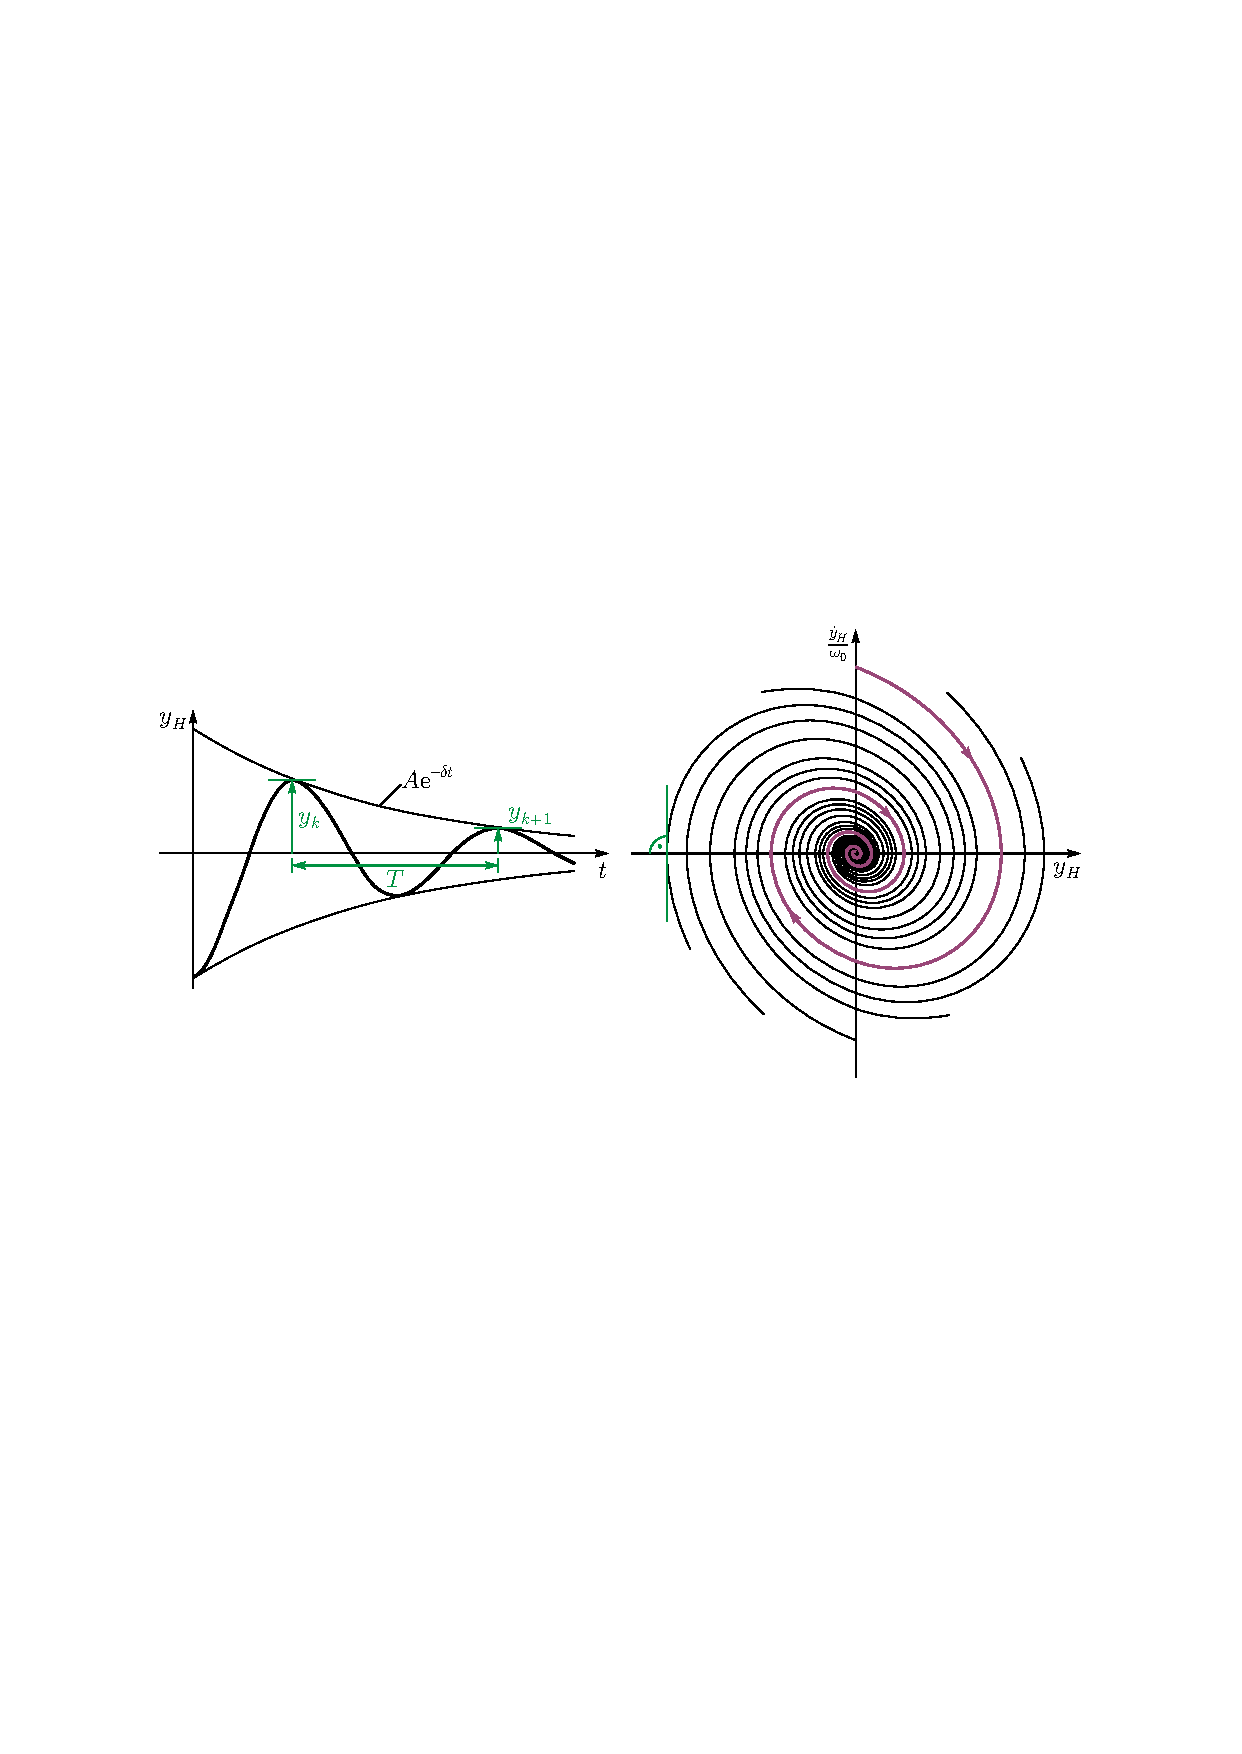
\includegraphics[width=\columnwidth]{grafiken/daempfung_d_0_1_1}
						$D = 0.17$
						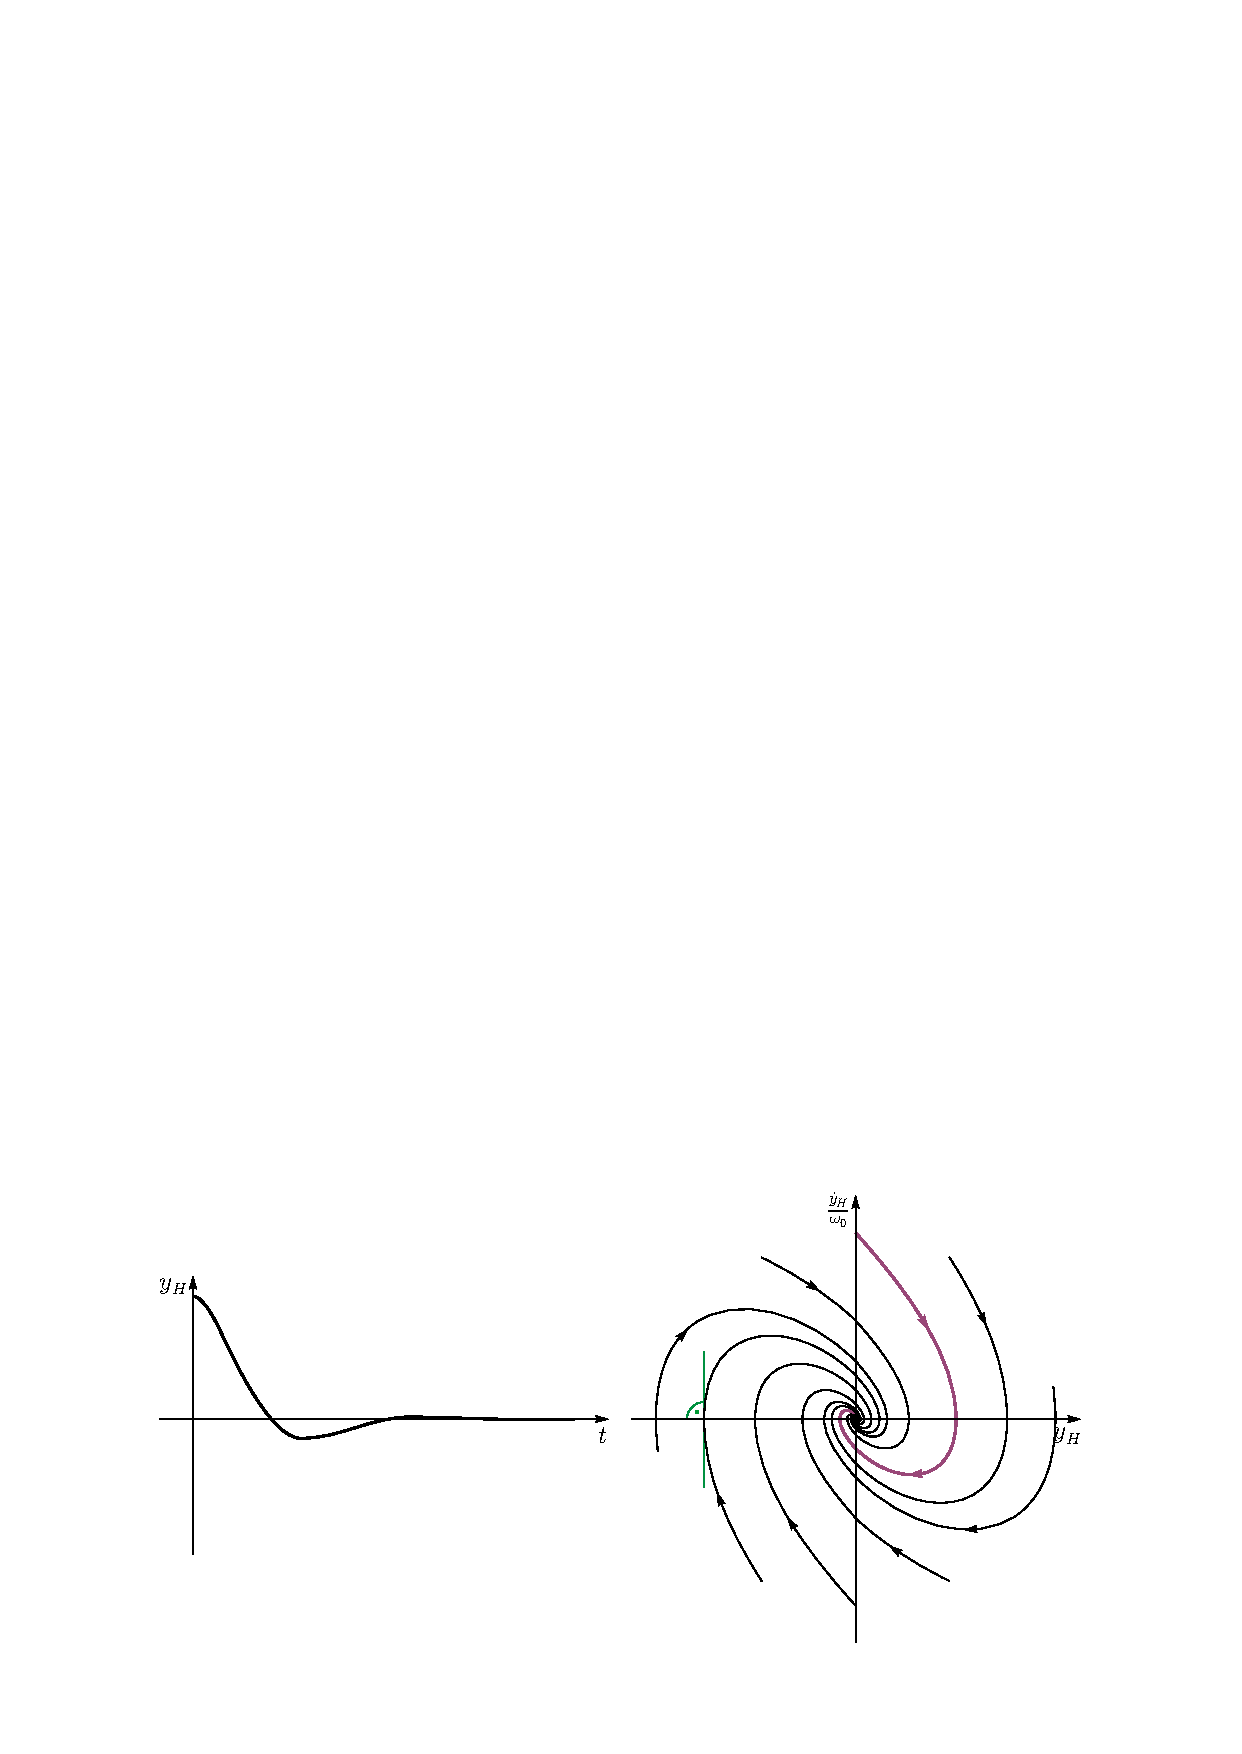
\includegraphics[width=\columnwidth]{grafiken/daempfung_d_0_1_2}
						$D = 0.5$
					\end{center}
					
					\paragraph{Logarithmisches Dekrement} % (fold)
						\[
							\Lambda := \delta T = \delta \frac{2 \pi}{\omega} = 2 \pi \frac{\delta}{\omega} = 2\pi \sqrt{\frac{D^2}{1-D^2}} = \ln \frac{y(t)}{y(t+T)}
						\]
						
						\[
							D = \sqrt{\frac{\Lambda^2}{\Lambda^2 + 4\pi^2}}
						\]
					% paragraph: Logarithmisches Dekrement (end)
				% subsubsection: Unterkritisch gedämpfte Schwingung $(D \in (0,1))$ (end)
				
				\subsubsection{Kritische Dämpfung $(D = 1)$} % (fold)
					
					\begin{empheq}[box=\shadowbox*]{equation*}
						\lambda_{1,2} = - \delta
					\end{empheq}
					
					\[
						y_h = t e^{\lambda t}
						\quad
						\dot{y}_h = \lambda t e^{\lambda t} + e^{\lambda t}
						\quad
						\ddot{y}_h = \lambda^2 t e^{\lambda t} + 2 \lambda e^{\lambda t}
					\]
					
					\begin{center}
						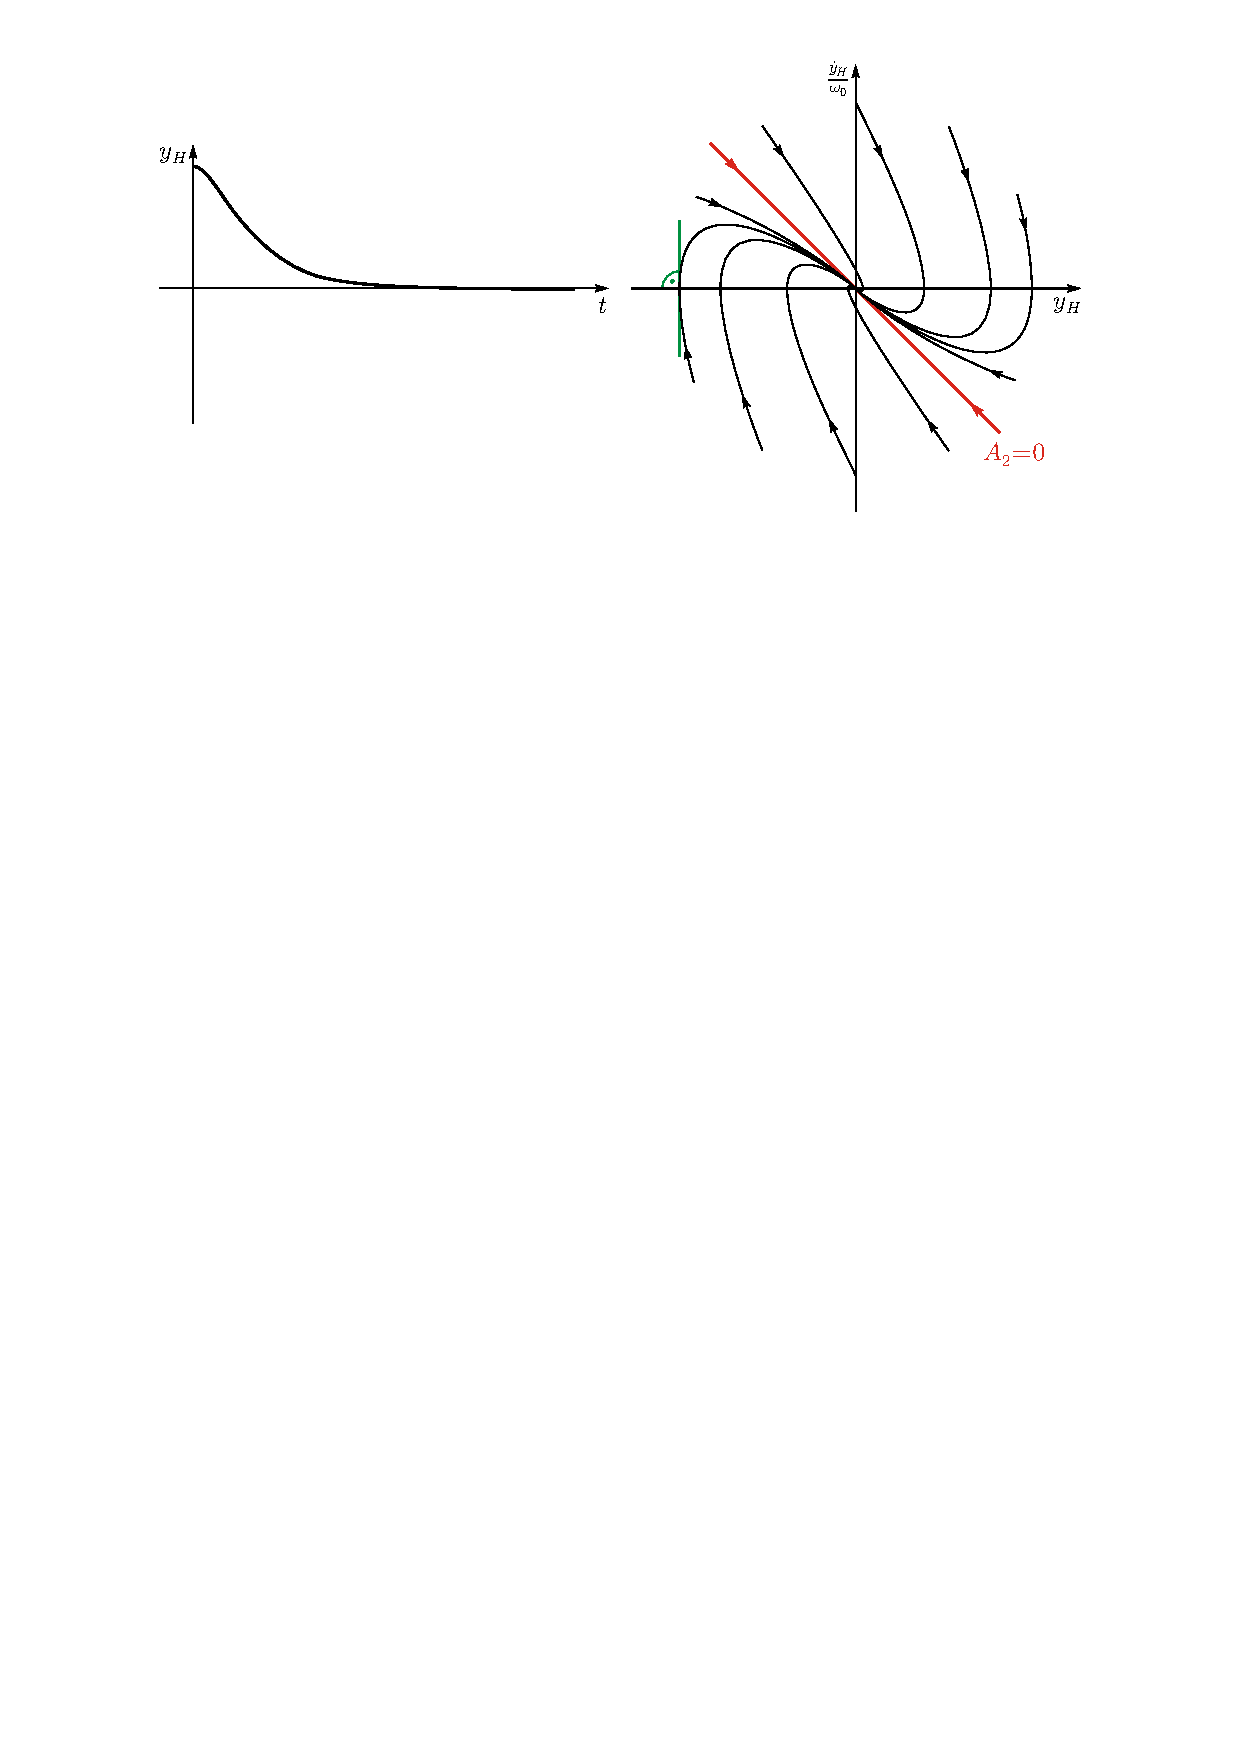
\includegraphics[width=\columnwidth]{grafiken/daempfung_d_1}
					\end{center}
				% subsubsection: Kritische Dämpfung (D=1) (end)
				
				\subsubsection{Überkritische Dämpfung $(D > 1)$} % (fold)
					
					\begin{empheq}[box=\shadowbox*]{equation*}
						\lambda_{1,2} = - \delta \pm \psi
					\end{empheq}
					wobei
					\[
						\psi^2 := \delta^2 - \omega_0^2 = \omega_0^2 (D^2 - 1) \qquad 0 < \psi < \delta
					\]
					
					\begin{align*}
						y_h(t) &= e^{-\delta t} (A_1 e^{\psi t} + A_2 e^{-\psi t}) \\
						&= e^{-\delta t} (B_1 \cosh \psi t + B_2 \sinh \psi t)
					\end{align*}
					wobei $B_{1,2} = \frac{1}{2}(A_1 \pm A_2)$
					
					\begin{center}
						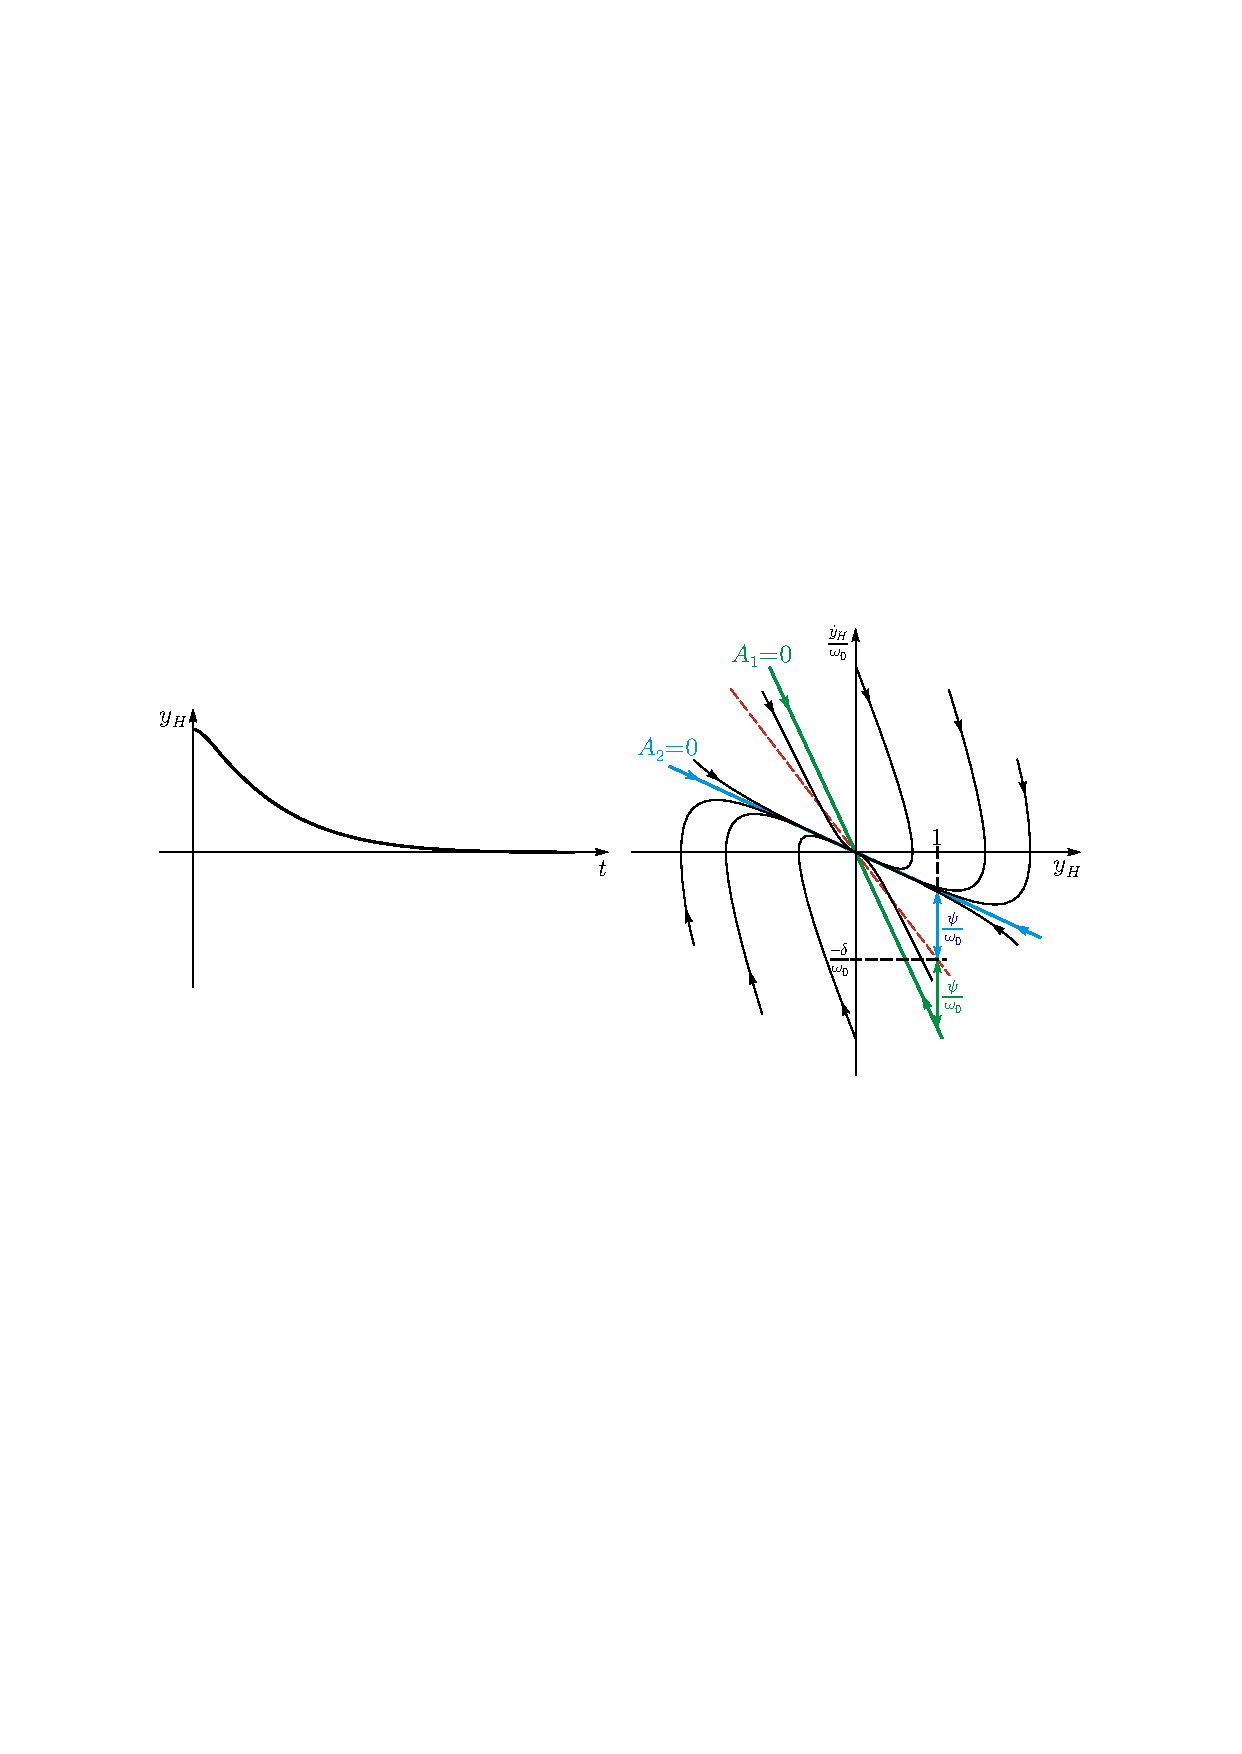
\includegraphics[width=\columnwidth]{grafiken/daempfung_d_g1}
						$D = 1.3$
					\end{center}
					
					\paragraph{Grenzfall $(D \to \infty)$} % (fold)
						
						\[
							\frac{\delta}{\omega_0} = 0 \qquad \frac{\psi}{\omega_0} = \sqrt{D^2 - 1} \qquad \psi \to \delta
						\]
						
						\begin{center}
							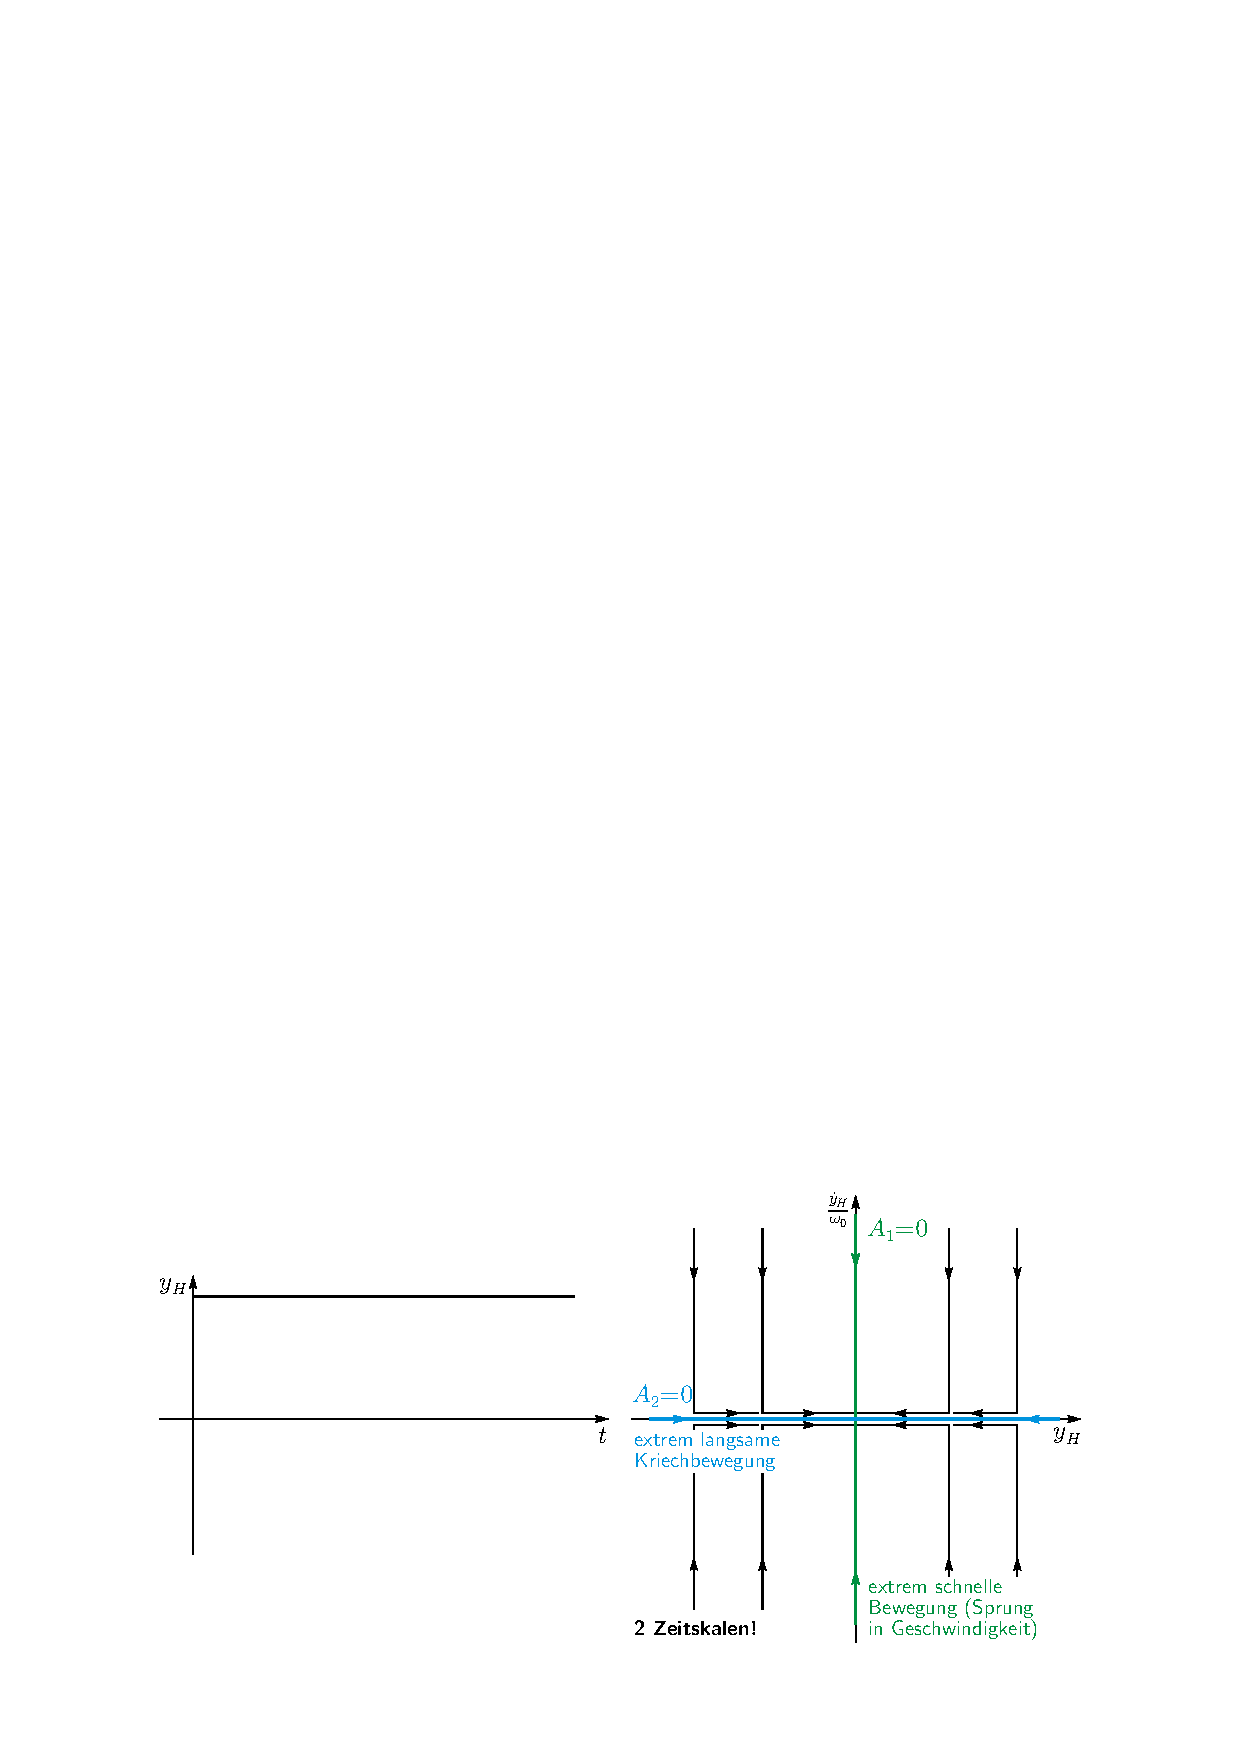
\includegraphics[width=\columnwidth]{grafiken/daempfung_d_infty}
						\end{center}
					% paragraph: Grenzfall (D $\to \infty$) (end)
				% subsubsection: Überkritische Dämpfung $\mathbf{}$ (end)
				
			% subsection: Dämpfung (end)
			
			\subsection{Lösung der inhomogenen Gleichung} % (fold)
				
				\subsubsection{Partikuläre Lösung} % (fold)
					
					\[
						m \ddot{y}_p + d \dot{y}_p + c y_p = \hat{F} \cos \Omega t \quad \forall t
					\]
					
					\begin{empheq}[box=\shadowbox*]{equation*}
						y_p (t) = \hat{y} \cos (\Omega t - \varphi)
					\end{empheq}
					
					\begin{gather*}
						\varphi = \psi \qquad \hat{y} = \hat{F} \cdot \frac{1}{r} \\
						r = m \cdot \omega_0^2 \cdot \sqrt{(1-\eta^2)^2 + (2D \eta)^2} \\
						\tan(\psi) = \frac{2D\eta}{1-\eta^2} \qquad \eta = \frac{\Omega}{\omega_0}
					\end{gather*}
					
					\begin{empheq}[box=\shadowbox*]{equation*}
						y_p (t) = \frac{\hat{F}}{m \omega_0^2} V \cos (\Omega t - \varphi)
					\end{empheq}
					
					\[
						V = \frac{1}{\sqrt{(1- \eta^2)^2 + (2D \eta)^2}} \qquad \varphi = \arctan \left(\frac{2D\eta}{1-\eta^2}\right)
					\]
				% subsubsection: Partikuläre Lösung (end)
				
				\subsubsection{Homogene Lösung} % (fold)
				
					Vgl.~\nameref{subsec:daempfung} auf Seite~\pageref{subsec:daempfung}.
					
					\begin{tabular}{ll@{}}
						\textbf{asymptotisch stabil} falls & $D > 0$ \\
						\textbf{grenzstabil} falls & $D = 0$
					\end{tabular}
				% subsubsection: Homogene Lösung (end)
				
			% subsection: Lösung der inhomogenen Gleichung (end)
		% section: Lineare Schwingungen mit einem Freiheitsgrad (end)
		\section{Lineare Schwingungen mit $f$ Freiheitsgraden} % (fold)
			\subsection{Vorbemerkungen} % (fold)
				\begin{tabular}{lll}
				\toprule
				Eigenschaft & Bedingung & Eigenwerte\\
				\midrule
				symmetrisch & $\mtrx{A}=\mtrx{A}^\transp$ & immer reel \\
				schiefsymmetrisch & $\mtrx{A}=-\mtrx{A}^\transp$ & rein imaginär \\
				positiv definit & $\vec{x}^\transp \mtrx{A} \vec{x} > 0 \quad \forall \vec{x} \neq 0$ & immer positiv \\
				positiv semidefinit & $\vec{x}^\transp \mtrx{A} \vec{x} \geq 0 \quad \forall \vec{x}$ & positiv oder 0\\
				\bottomrule
				\end{tabular}
				
			% subsection: Vorbemerkungen (end)
			
			\subsection{Struktur} % (fold)
				\begin{empheq}[box=\shadowbox*]{equation*}
					\mtrx{M} \ddot{\vec{y}} + \mtrx{B} \dot{\vec{y}} + \mtrx{C} \vec{y} = \vec{f}(t)
				\end{empheq}
				
				$\mtrx{M},\mtrx{B},\mtrx{C} \in \R^{f \times f}$ sind konstant.
				
				\subsubsection{M-D-G-K-N-System} % (fold)
					\begin{empheq}[box=\shadowbox*]{equation*}
						\mtrx{M} \ddot{\vec{y}} + (\mtrx{D}+\mtrx{G}) \dot{\vec{y}} + (\mtrx{K}+\mtrx{N}) \vec{y} = \vec{f}(t)
					\end{empheq}
					
					\begin{center}
						\begin{tabular}{ll}
						\toprule
						$\mtrx{M} = \mtrx{M}^\transp$ & Massenmatrix \\
						\vspace{2mm}
						 & (invertierbar) \\
						\vspace{2mm}
						$\mtrx{D} = \mtrx{D}^\transp := \frac{1}{2} (\mtrx{B}+\mtrx{B}^\transp)$ & Dämpfungsmatrix \\
						$\mtrx{G} = -\mtrx{G}^\transp := \frac{1}{2} (\mtrx{B}-\mtrx{B}^\transp)$ & Gyro-Matrix \\
						\vspace{2mm}
						 & (Coriolistherme) \\
						\vspace{2mm}
						$\mtrx{K} = \mtrx{K}^\transp :=\frac{1}{2} (\mtrx{C}+\mtrx{C}^\transp)$ & Stefigkeitsmatrix \\
						$\mtrx{N} = -\mtrx{N}^\transp := \frac{1}{2} (\mtrx{C}-\mtrx{C}^\transp)$ & Matrix der \\ & zirkulierenden Kräfte \\
						\bottomrule
						\end{tabular}
					\end{center}
					
					\paragraph{Zustandsraumdarstellung} % (fold)
						\begin{align*}
							\begin{bmatrix}
								\vec{\dot{y}} \\ \ddot{\vec{y}}
							\end{bmatrix}
							= &
							\begin{bmatrix}
								0 & \mtrx{I} \\
								-\mtrx{M}^{-1} (\mtrx{K}+\mtrx{N}) & -\mtrx{M}^{-1} (\mtrx{D}+\mtrx{G})
							\end{bmatrix}
							\cdot
							\begin{bmatrix}
								\vec{y} \\ \dot{\vec{y}}
							\end{bmatrix}
							\\ &+
							\begin{bmatrix}
								0 \\ \mtrx{M}^{-1} \vec{f}(t)
							\end{bmatrix}
						\end{align*}
					% paragraph: Zustandsraumdarstellung (end)
				% subsubsection: M-D-G-K-N-System (end)
			% subsection: Struktur (end)
			
			\subsection{M-K-System} % (fold)
				\[
					\mtrx{D}=\mtrx{G}=\mtrx{N}=0 \ \Rightarrow \ \mtrx{M} \ddot{\vec{y}} + \mtrx{K} \vec{y} = \vec{f}(t)
				\]
				\begin{empheq}[box=\shadowbox*]{equation*}
					\vec{y}_h = \vec{u} \cdot e^{\lambda t} \qquad 
					\dot{\vec{y}}_h = \lambda \cdot \vec{u} \cdot e^{\lambda t} \qquad
					\ddot{\vec{y}}_h = \lambda^2 \cdot \vec{u} \cdot e^{\lambda t}
				\end{empheq}
				\[
					(\mtrx{M} \lambda^2 + \mtrx{K}) \cdot \vec{u} = 0
				\]
				
				\subsubsection{Semipositiv definite Matrix K} % (fold)
				
					\begin{description}
						\item[falls $\lambda_{1,2} = \pm \iu \omega_0 \ (\omega_0 > 0)$:]
						\[
							\vec{y}_1 = \vec{u}_1 e^{\iu \omega_0 t} \qquad \vec{y}_2 = \vec{u}_2 e^{-\iu \omega_0 t}
						\]
						
						\item[falls $\lambda_{1,2} = 0$:]
						\[
							\vec{y}_1 = \vec{u}_1 \ , \quad \vec{y}_2 = t \vec{u}_1
						\]
					\end{description}
					
				% subsubsection: Semipositiv definite Matrix $\mathbf{}$ (end)
				
				\subsubsection{Positiv definite Matrix K} % (fold)
					
					$\mtrx{U} \in \R^{f \times f}$ ist die Matrix der Pseudoeigenvektoren.
					
					\[
						\mtrx{U}^\transp \mtrx{M}\mtrx{U} =: \diag{\{\mu_i\}} \qquad \mtrx{U}^\transp \mtrx{K}\mtrx{U} =: \diag{\{\kappa_i\}}
					\]
					
					\paragraph{Modale Koordinaten} % (fold)
						\[
							\vec{\xi}(t) = \mtrx{U}^{-1} \vec{y}(t) \, , \quad \ddot{\vec{y}} = \mtrx{U} \ddot{\vec{\xi}} = \sum \vec{u}_i \ddot{\xi}_i (t)
						\]
						führt zu
						\begin{gather*}
							\mu_i \ddot{\xi}_1 + \kappa_i \xi_i = \beta_i (t) \qquad \ddot{\xi}_i + \omega_{0_i}^2 \xi_i = \frac{\beta_i (t)}{\mu_i}
						\end{gather*}
					% paragraph: Modale Koordinaten (end)
					
				% subsubsection: Positiv definite Matrix $\mathbf{}$ (end)
			% subsection: M-K-System (end)
			\subsection{M-K-System mit Dämpfung nach Bequemlichkeit} % (fold)
				\[
					\mtrx{M} \ddot{\vec{y}} + \mtrx{D} \dot{\vec{y}} + \mtrx{K} \vec{y} = \vec{f}(t)
				\]
				
				\begin{align*}
					\mu_i \ddot{\xi}_i + (\alpha \mu_i + \beta \kappa_i) \dot{\xi_i} + \kappa_i \xi_i &= \beta_i(t) \\
					\ddot{\xi}_i + 2\delta_i \dot{\xi_i} +\omega_{0_i}^2 \xi_i &= \frac{\beta_i(t)}{\mu_i}
				\end{align*}
				mit $\omega_{0_i}^2 = \frac{\kappa_i}{\mu_i}$ und $\delta_i = \frac{1}{2} (\alpha + \beta \omega_{0_i}^2)$.
				
				\paragraph{Bequemlichkeitshypothese:} % (fold)
					\[
						\mtrx{D}:= \alpha \mtrx{M} + \beta \mtrx{K} \qquad \alpha,\beta \in \R \quad (\text{oft }\alpha = 0)
					\]
				% paragraph: Bequemlichkeitshypothese: (end)
			% subsection: M-K-System mit Dämpfung nach Bequemlichkeit (end)
			\subsection{Stabilität des MDGKN-Systems} % (fold)
				\begin{tabular}{@{}ll@{}}
					\vspace{2mm}
					\textbf{asymptotisch stabil} falls & $\Re(\lambda_i) < 0 \quad \forall i$ \\
					\textbf{grenzstabil} falls & $\exists \Re(\lambda_i) > 0$
				\end{tabular}
				
			% subsection: Stabilität des MDGKN-Systems (end)
		% section: Lineare Schwingungen mit $f$ Freiheitsgraden (end)
		\section{Die Wellengleichung} % (fold)
			\subsection{Bewegungsgleichung spezieller 1-D Kontinua} % (fold)
				\paragraph{Wellengleichung:} % (fold)
					(PDGL 2. Ordnung)
					\[
						u_{tt}(x,t) = c^2 u_{xx} (x,t)
					\]
					mit konstanter \emph{Wellengeschwindigkeit} $c \unit{\metre\per\second}$ und
					\begin{align*}
						u&: \text{ Auslenkung} \\
						u_x&: \text{ Spannung/Dehnung} \\
						u_t&: \text{ Geschwindigkeit}
					\end{align*}
				% paragraph: Wellengleichung: (end)
			% subsection: Bewegungsgleichung spezieller 1-D Kontinua (end)
			\subsection{Allgemeine Lösung der Wellengleichung} % (fold)
				\[
					u(x,t) = \underbrace{f(\overbrace{\vphantom{\frac{1}{2}} x-ct}^{\xi})}_{u_f: \text{ Rechtswelle}} + \underbrace{g(\overbrace{\vphantom{\frac{M}{2}} x+ct}^{\eta})}_{u_g: \text{ Linkswelle}}
				\]
				
				\paragraph{Umrechnung von Spannung und Geschwindigkeiten} % (fold)
					\[
						u_{f,t} = -c \, u_{f,x} \qquad u_{g,t} = c \, u_{g,x}
					\]
				% paragraph: Umrechnung von Spannung und Geschwindigkeiten (end)
				
				\begin{center}
					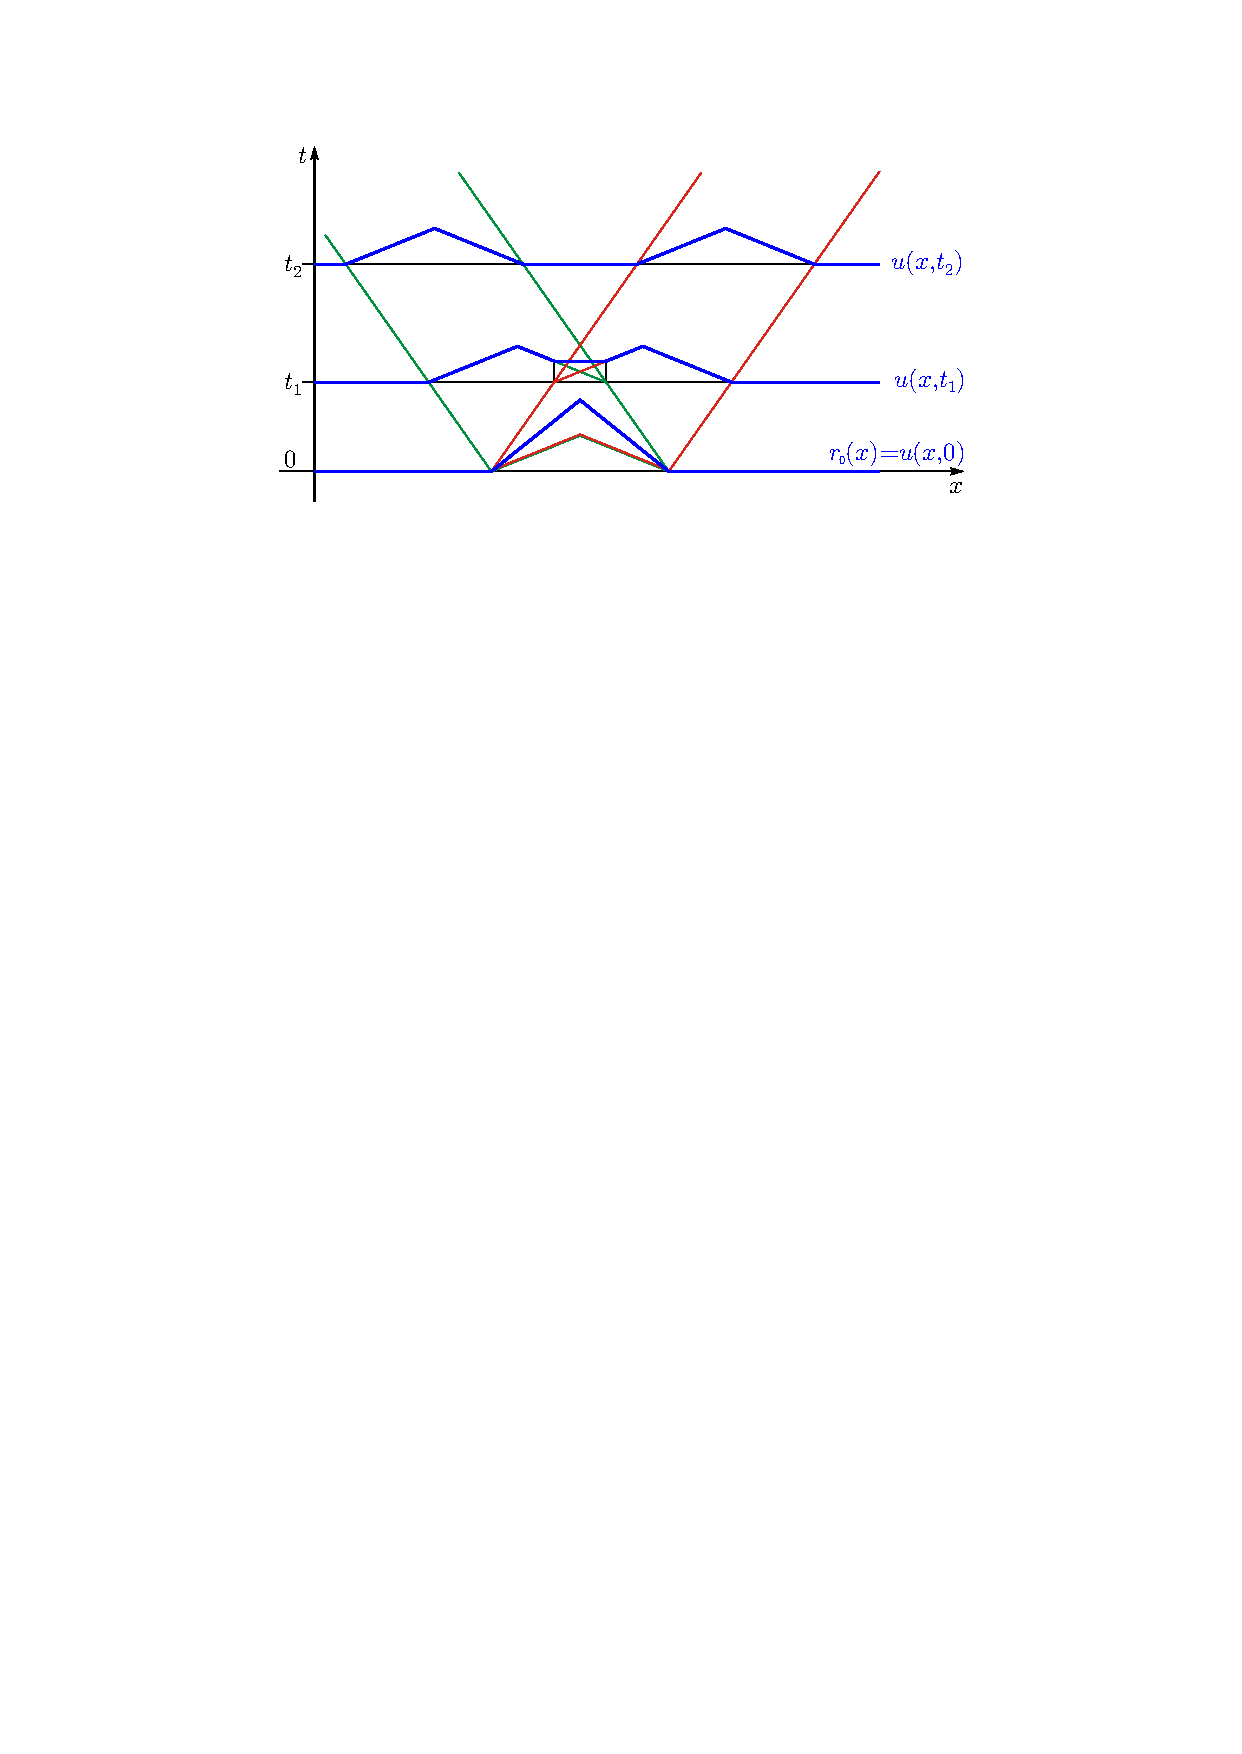
\includegraphics[width=\columnwidth]{grafiken/wellenausbreitung}
				\end{center}
			% subsection: Allgemeine Lösung der Wellengleichung (end)
			
			\subsection{Randbedingungen} % (fold)
				\paragraph{Eingespanntes Ende:} % (fold)
					$u(x=0,t) \equiv 0 \quad \forall t \in \R$
					
					\begin{itemize}
						\item Rechtswelle $\Longleftrightarrow$ Linkswelle
						\item Druckwelle $\Longleftrightarrow$ Druckwelle
					\end{itemize}
					
					\begin{center}
						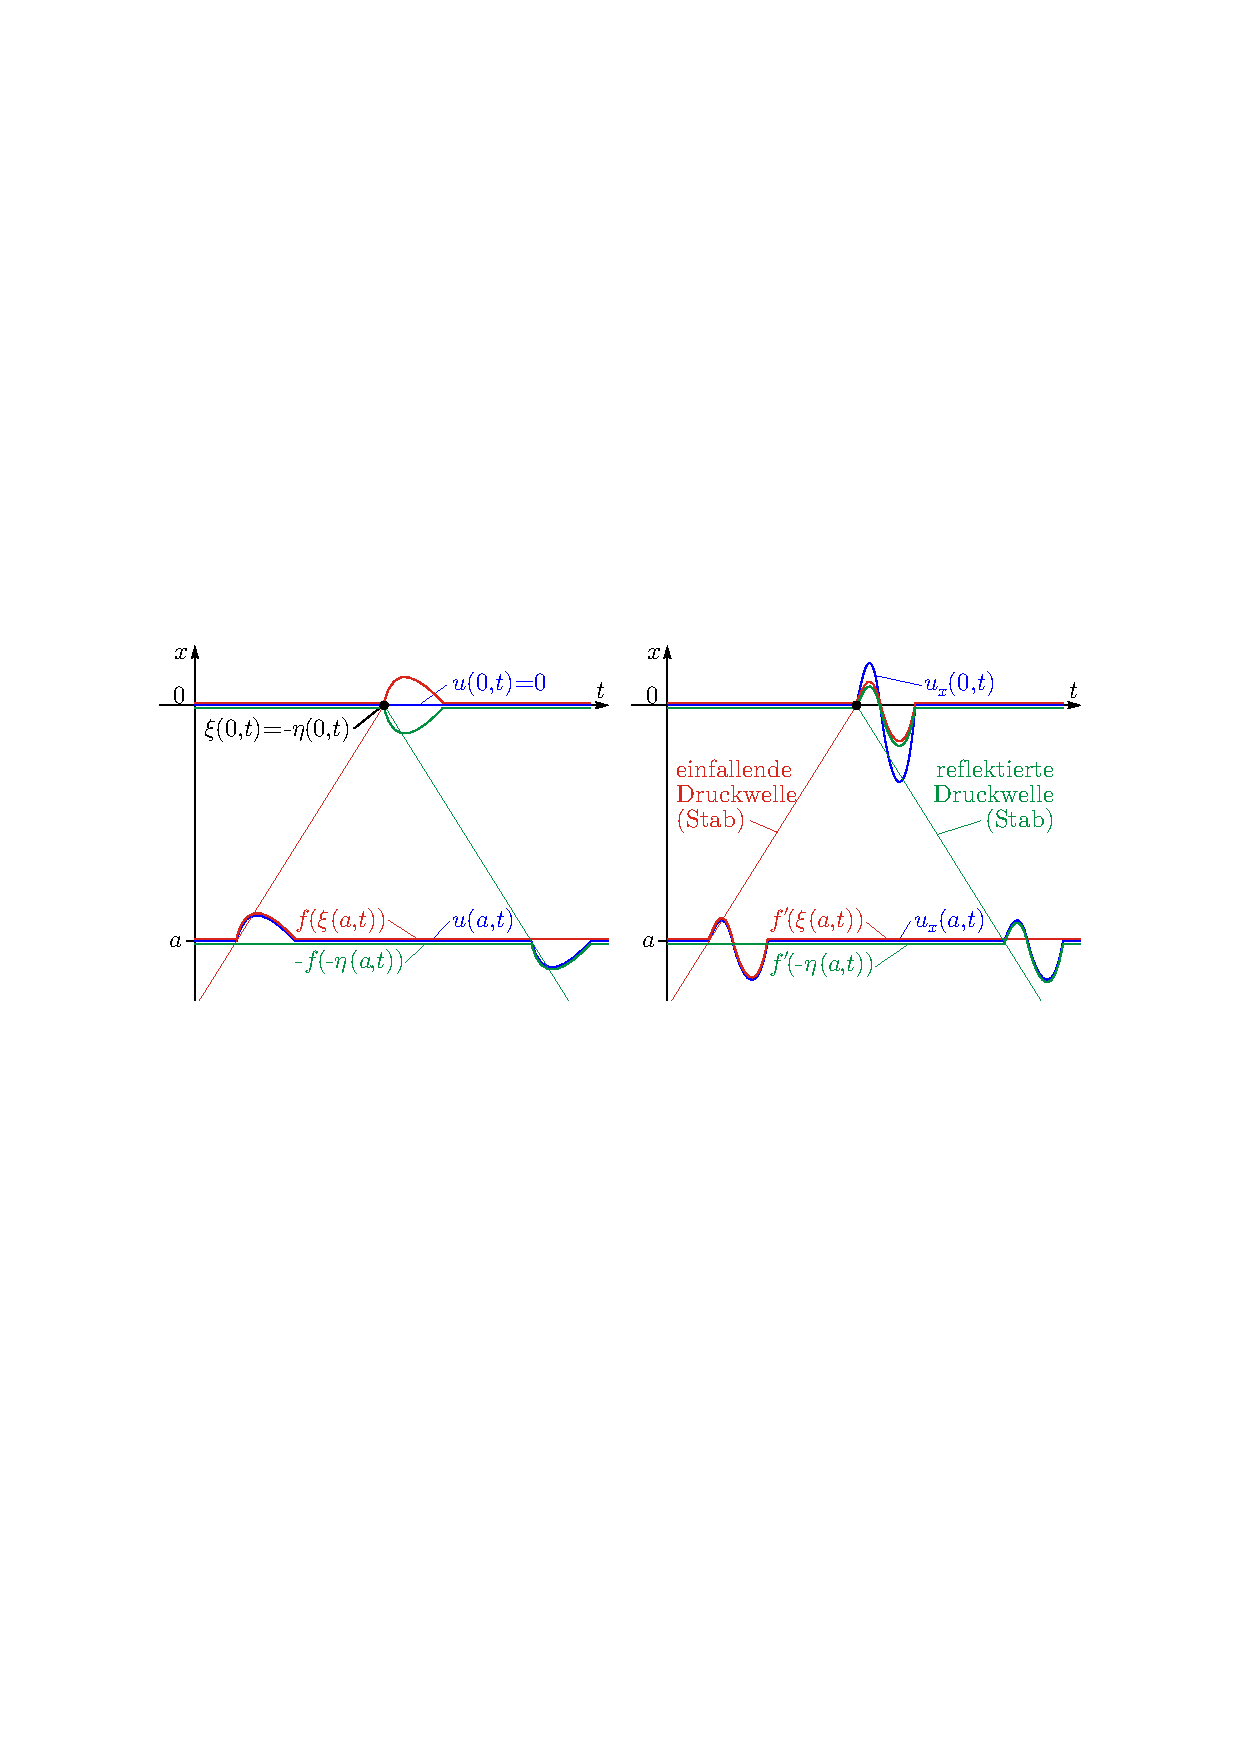
\includegraphics[width=\columnwidth]{grafiken/reflexion_eingespanntes_ende}
					\end{center}
				% paragraph: Eingespanntes Ende: (end)
				
				\paragraph{Freies Ende:} % (fold)
					$u_x(x=0,t) \equiv 0$
					
					\begin{itemize}
						\item Rechtswelle $\Longleftrightarrow$ Rechtswelle
						\item Druckwelle $\Longleftrightarrow$ Zugwelle
					\end{itemize}
					
					\begin{center}
						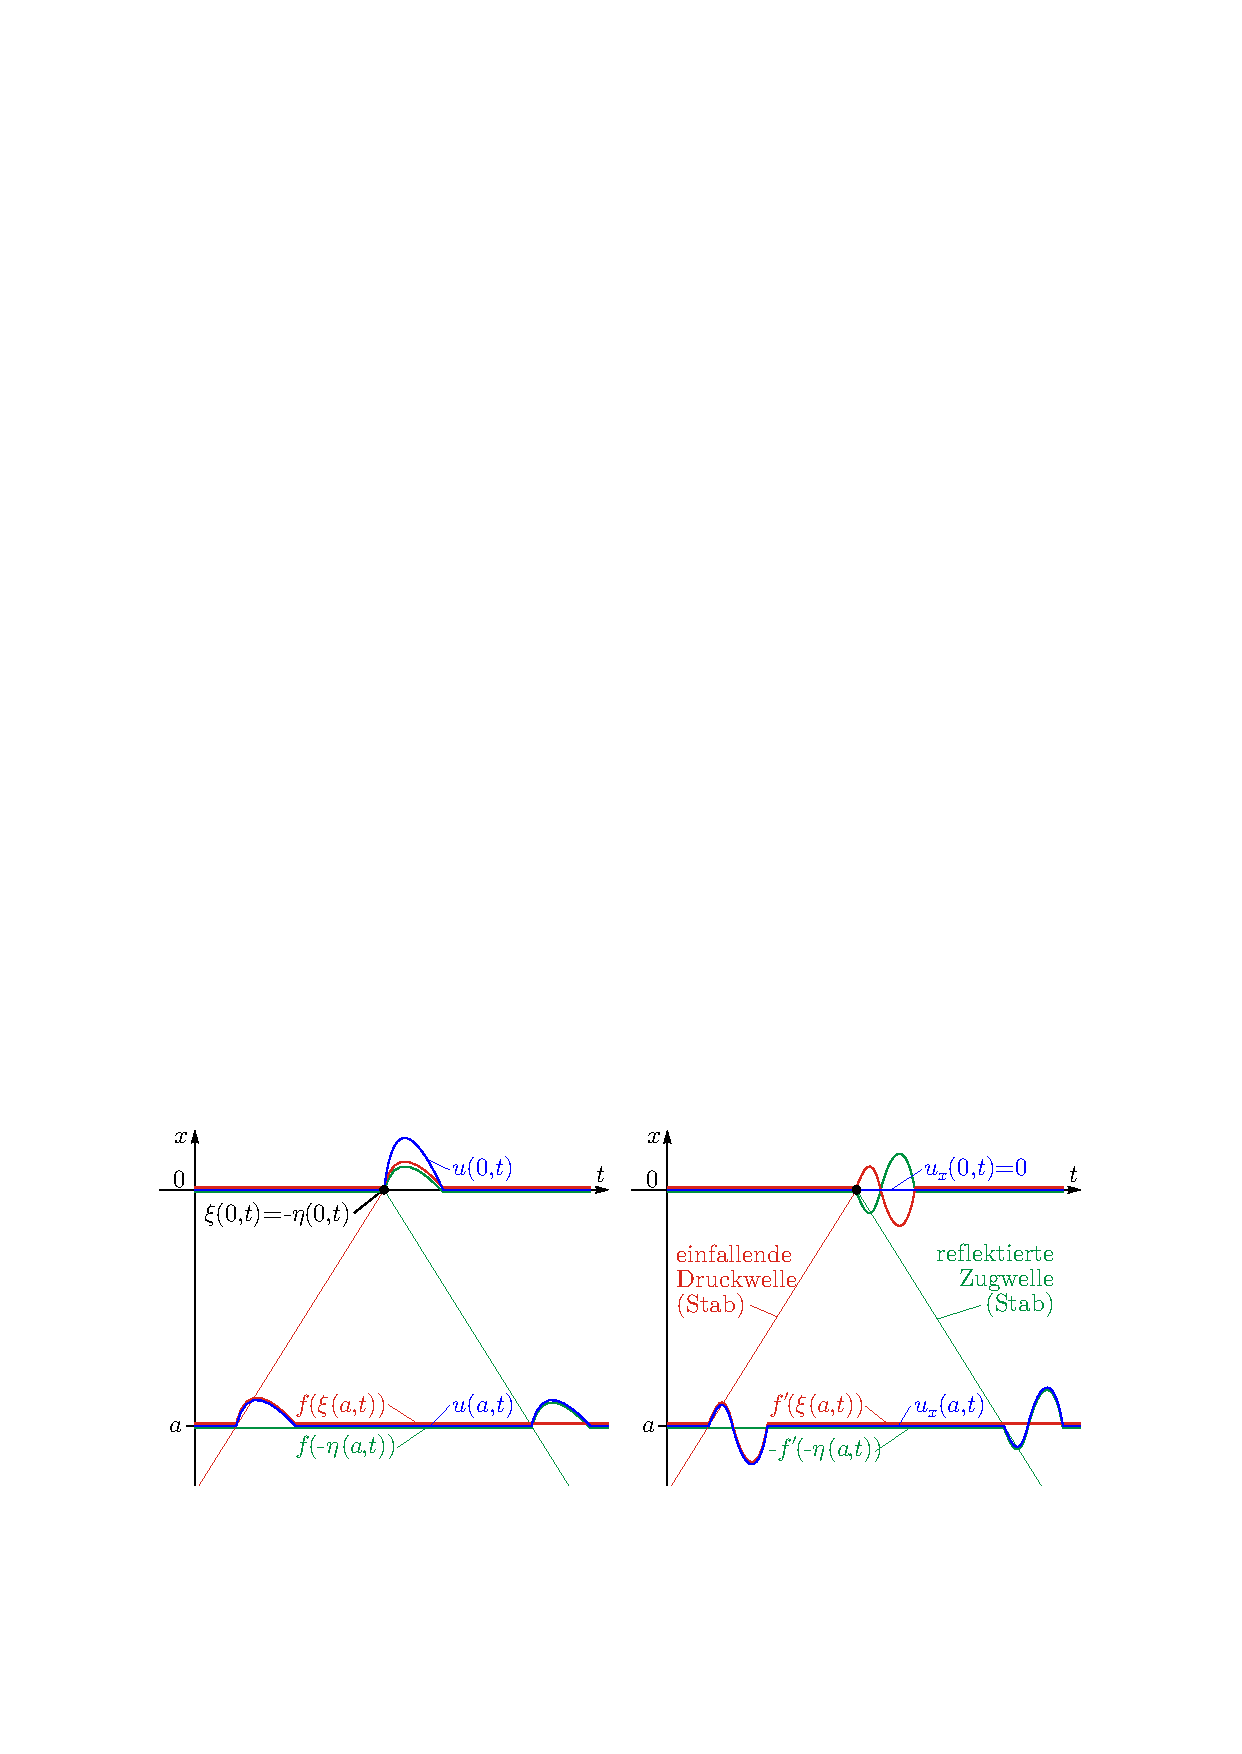
\includegraphics[width=\columnwidth]{grafiken/reflexion_freies_ende}
					\end{center}
				% paragraph: Freies Ende: (end)
			% subsection: Randbedingungen (end)
			\subsection{Stehende Wellen} % (fold)
				\[
					u(x,t) = u_f(\xi) + u_g(\eta) = 
					\underbrace{w(x)\vphantom{\frac{M}{2}}}_{\mathclap{\text{Ortsfunktion}}} \cdot \overbrace{q(t) \vphantom{\frac{M}{2}}}^{\mathclap{\text{Zeitfunktion}}}
				\]
				\emph{Ortsfunktion} (auch Amplitudenfunktion) beschreibt die Form der stehenden Welle. \emph{Zeitfunktion} ist das zeitliche pulsieren der stehenden Welle.
				
				\paragraph{Separation der Variablen:} % (fold)
					\[
						\frac{\ddot{q}(t)}{q(t)} = c^2 \, \frac{w''(x)}{w(x)} = -\omega^2
					\]
				% paragraph: Separation der Variablen: (end)
				
				\paragraph{Lösen der Gleichung:} % (fold)
					
					\[
						u(x,t) = \sum_j \underbrace{
							\widetilde A_j \sin \left(
								\frac{\omega_j}{c} \xi + \varphi_j
							\right)
						}_{f_j(\xi)} + \underbrace{
							\widetilde B_j \sin \left(
								\frac{\omega_j}{c} \eta + \psi_j
							\right)
						}_{g_j(\eta)}
					\]
				
					wobei $\widetilde A,\, \widetilde B,\, \varphi,\, \psi$ und $\omega$ beliebige Konstanten sind, die durch \emph{Anfangs- und Randbedingungen} bestimmt werden.
				% paragraph: Lösen der Gleichung: (end)
				\paragraph{Wellenzahl:} % (fold)
					$k:= \frac{\omega}{c}$
				% paragraph: Wellenzahl: (end)
				\paragraph{Wellenlänge:} % (fold)
					$\lambda := \frac{2 \pi}{k}$
				% paragraph: Wellenlänge: (end)
			% subsection: Stehende Wellen (end)
		% section: Die Wellengleichung (end)
		\section{Kinematik} % (fold)
			\subsection{Koordinaten \& Vektoren} % (fold)
				\begin{description}
					\item[Inertialsysteme:] bezeichnet mit $I$, \emph{unbeschleunigt}
					\item[Körperfeste Koordinatensysteme] bezeichnet mit $K$, erhält man, indem man Koordinatenachsen an einen Starrkörper festbindet
				\end{description}
				Alle Koordinatensysteme entstehen durch Drehung von $I$.
				
				Strikte Unterscheidung zwischen dem ``Pfeil'' $\vec{c} \in V$ (koordinatenfrei) und der koordinatenbehafteten Darstellung $\vecin{c}{B} \in \R^3$.
				
				\paragraph{Koordinatenabbildung:} % (fold)
					\begin{empheq}[box=\shadowbox*]{equation*}
						\vecin{c}{B} = \trafo{K}{B} (\vec{c}) \qquad \vec c = \trafo{K}{B}^{-1} (\vecin{c}{B})
					\end{empheq}
				% paragraph: Koordinatenabbildung: (end)
			% subsection: Koordinatensysteme, Vektoren und Koordinaten (end)
			
			\subsection{Koordinatentransformation} % (fold)
				\begin{empheq}[box=\shadowbox*]{equation*}
					\vecin{c}{D} = \trafo{K}{D} \trafo{K}{B}^{-1} \vecin{c}{B} \qquad
					\vecin{c}{D} = \trafo{A}{DB} \cdot \vecin{c}{B}
				\end{empheq}
				$\trafo{A}{DB}$ ist die Transformationsmatrix von $B \to D$.
				\[
					\trafo{A}{DB} = \left[
						\vecin{e}{D}_x^B \quad \vecin{e}{D}_y^B \quad \vecin{e}{D}_z^B
					\right]
				\]
				\begin{empheq}[box=\shadowbox*]{equation*}
					\trafo{A}{DB}^\transp = \trafo{A}{DB}^{-1} = \trafo{A}{BD} \qquad \trafo{A}{BD} \cdot \trafo{A}{DB} = \mtrx{I}
				\end{empheq}
				
				\subsubsection{Elementardrehungen} % (fold)
					\begin{gather*}
						\trafo{A}{DB} = \begin{bmatrix}
							1 & 0 & 0 \\
							0 & \operatorname c \alpha & \operatorname s \alpha \\
							0 & -\operatorname s \alpha & \operatorname c \alpha
						\end{bmatrix}
						\quad
						\trafo{A}{DB} = \begin{bmatrix}
							\operatorname c \beta & 0 & -\operatorname s \beta \\
							0 & 1 & 0 \\
							\operatorname s \beta & 0 & \operatorname c \beta
						\end{bmatrix} \\
						\trafo{A}{DB} = \begin{bmatrix}
							\operatorname c \gamma & \operatorname s \gamma & 0 \\
							-\operatorname s \gamma & \operatorname c \gamma & 0 \\
							0 & 0 & 1
						\end{bmatrix}
					\end{gather*}
					\[
						\trafo{A}{14} = \trafo{A}{12} \cdot \trafo{A}{23} \cdot \trafo{A}{34}
					\]
				% subsubsection: Elementardrehungen (end)
			% subsection: Koordinatentransformation (end)
			\subsection{Drehgeschwindigkeit zwischen zwei Koordinatensystemen} % (fold)
				\label{subsec:drehgeschwindigkeit_zwischen_zwei_koordinatensystemen}
				\[
					\vec{a} = \begin{pmatrix}
						a_1 \\ a_2 \\ a_3
					\end{pmatrix},
					\quad
					\widetilde{\mtrx{a}} := \begin{bmatrix}
						0 & -a_3 & a_2 \\
						a_3 & 0 & -a_1 \\
						-a_2 & a_1 & 0
					\end{bmatrix},
					\quad
					\vec{a} \times \vec{b} \equiv \widetilde{\mtrx{a}}\cdot \vec{b}
				\]
				
				\paragraph{Winkelgeschwindigkeit:} % (fold)
					\momegain{BD}{B} ist die Winkelgeschwindigkeit von $B$ gegenüber $D$ bezüglich dem System $B$:
					\[
						\momegain{BD}{B} = \trafo{\dot A}{BD} \cdot \trafo{A}{BD}^\transp \qquad \trafo{\widetilde \omega}{DB} = -\trafo{\widetilde \omega}{BD}
					\]
				% paragraph: Winkelgeschwindigkeit: (end)
				
				\paragraph{Elementargeschwindigkeiten} % (fold)
					\[
						\omegain{BD}{B} = \begin{pmatrix}
							\dot \alpha \\ 0 \\ 0
						\end{pmatrix},
						\quad
						\omegain{BD}{B} = \begin{pmatrix}
							0 \\ \dot \beta \\ 0
						\end{pmatrix},
						\quad
						\omegain{BD}{B} = \begin{pmatrix}
							0 \\ 0 \\ \dot \gamma
						\end{pmatrix}
					\]
				% paragraph: Elementargeschwindigkeiten (end)
				
				\paragraph{Transformation von Drehgeschwindigkeiten:} % (fold)
					\[
						\momegain{BD}{D} = \trafo{A}{DB} \cdot \momegain{BD}{B} \cdot \trafo{A}{DB}^\transp \qquad
						\omegain{BD}{D} = \trafo{A}{DB} \cdot \omegain{BD}{B}
					\]
				% paragraph: Transformation von Drehgeschwindigkeiten (end)
				
				\paragraph{Gesamtwinkelgeschwindigkeit:} % (fold)
					$\trafo{\omega}{14} = \trafo{\omega}{12} + \trafo{\omega}{23} + \trafo{\omega}{34}$
				% paragraph: Gesamtwinkelgeschwindigkeit (end)
			% subsection: Drehgeschwindigkeit zwischen zwei Koordinatensystemen (end)
			
			\subsection{Ableitungen von Vektoren in bewegten Systemen} % (fold)
				\begin{align*}
					\vec{c} &: \text{ ``Pfeil''} \\
					\dot{\vec{c}} &: \text{ zeitliche Ableitung von } \vec{c} \\
					_B (\dot{\vec{c}}) &: \text{ Koordinaten von } \dot{\vec{c}} \text{ in der Basis } B \\
					(\vecin{c}{B})\highdot \equiv \vecin{\dot c}{B} &: \text{ zeitliche Ableitung von } \vecin{c}{B}
				\end{align*}
				Im Inertialsystem gilt:  $_{I}(\dot{\vec{c}}) \equiv \vecin{\dot c}{I} \equiv (\vecin{c}{I})\highdot$
				
				\paragraph{Eulersche Differentiationsregel:} % (fold)
					\begin{empheq}[box=\shadowbox*]{equation*}
						_B(\dot{\vec c}) = {}_B\dot{\vec c} + \omegain{IB}{B} \times \vecin{c}{B}
					\end{empheq}
					wobei \omegain{IB}{B} die Drehgeschwindigkeit des Systems $B$ relativ zu $I$, dargestellt in $B$, ist.
				% paragraph: Eulersche Differentiationsregel: (end)
			% subsection: Ableitungen von Vektoren in bewegten Systemen (end)
			
			\subsection{Kinematische Grössen von Starrkörpern} % (fold)
				\begin{center}
					\begin{tabular}{r@{$\:$}c@{$\:$}ll}\toprule
					\multicolumn{3}{c}{Symbol} & Geometrische Bedeutung \\\midrule
					$\bVec{r}_{AB}$&$\in$&$V$& Ortsvektor vom Punkt $A$ zum Punkt $B$ \\
					$\bVec{v}_B $&$\in$&$V$& (absolute) Geschwindigkeit des Punktes $B$ \\
					$\bVec{a}_B $&$\in$&$V$&  (absolute) Beschleunigung des Punktes $B$ \\
					$\bVec{\Omega}$&$\in$&$V$&  (absolute) Drehgeschwindigkeit des Körpers \\
					$\bVec{\Psi} $&$\in$&$V$&  (absolute) Drehbeschleunigung des Körpers
					\\\bottomrule
					\end{tabular}
				\end{center}
				\[
					\ddot{\vec r}_{AB} = \dot{\vec v}_B - \dot{\vec v}_A = \vec a_B - \vec a_A \quad , \qquad \dot{\vec \Omega} = \vec{\Psi}
				\]
			% subsection: Kinematische Grössen von Starrkörpern (end)
			
			\subsection{Berechnung von Geschwindigkeiten} % (fold)
				\begin{align*}
					\vec v_P       &= \vec v_A + \dot{\vec r}_{AP} \\
					\vecin{v}{B}_P &= \vecin{v}{B}_A + {}_B(\dot{\vec r}_{AP})
				\end{align*}
				$\Rightarrow$ Geschwindigkeit von $P$ in der Basis $B$:
				\begin{empheq}[box=\shadowbox*]{equation*}
					\vecin{v}{B}_P = \vecin{v}{B}_A + {}_B\dot{\vec r}_{AP} + \omegain{IB}{B} \times \vecin{r}{B}_{AP}
				\end{empheq}
				
				\paragraph{Starrkörperformel für Geschwindigkeiten:} % (fold)
					Es gilt ${}_K \dot{\vec r}_{PQ} \equiv 0$ und $\omegain{IK}{K} \equiv \vecin{\Omega}{K}$ und somit
					\begin{empheq}[box=\shadowbox*]{equation*}
						\vec v_Q = \vec v_P + \vec \Omega \times \vec r_{PQ}
					\end{empheq}
				% paragraph: Starrkörperformel: (end)
			% subsection: Berechnung von Geschwindigkeiten (end)
			
			\subsection{Berechnung von Beschleunigungen} % (fold)
				\begin{empheq}[box=\shadowbox*]{equation*}
					\vecin{\Psi}{B} = {}_B \dot{\vec \Omega} + \omegain{IB}{B} \times \vecin{\Omega}{B}
					%\Longleftrightarrow
					%{}_B(\dot{\vec c})\highdot = {}_B \ddot{\vec c} + \omegain{IB}{B} \times {}_B\dot{\vec c}
				\end{empheq}
				\paragraph{Spezialfälle:} % (fold)
					$
						\vecin{\Psi}{I} = {}_I \dot{\vec \Omega}
						\quad, \qquad
						\vecin{\Psi}{K} = {}_K \dot{\vec \Omega}
					$
				% paragraph: Spezialfälle: (end)
				
				\paragraph{Starrkörperformel für Beschleunigungen:} % (fold)
					\begin{empheq}[box=\shadowbox*]{equation*}
						\vec a_Q = \vec a_P + \vec \Psi \times \vec r_{PQ} + \vec \Omega \times (\vec \Omega \times \vec r_{PQ})
					\end{empheq}
				% paragraph: Starrkörperformel für Beschleunigungen: (end)
			% subsection: Berechnung von Beschleunigungen (end)
		% section: Kinematik (end)
		\section{Allgemeine Kinetik} % (fold)
			\subsection{Resultierende Kräfte/Trägheitsterme} % (fold)
				
				Resultierende äussere Kraft:\[
					\vec F^a := \int_K \diff \vec F^a
				\]
				
				Resultierendes äusseres Moment bezüglich $O$:\[
					\vec M_O^a := \int_K \vec \xi \times \diff \vec F^a + \diff \vec M^a
				\]
					\hspace{.5\columnwidth}
					\resizebox{.5\columnwidth}{!}{
						\begin{tikzpicture}[>=latex,scale=.9]

\coordinate (rect) at (-.2,.2);
\coordinate (rCenter) at (2.3,1.6);

\draw[interface] (-0.3,0) -- (.3,0);
\draw (0,0) -- (0,.5);
\fill (0, .5) circle (1pt) node[left] {$O$} ;

\path[draw,scale=1.7,shift={(1.1,1)},rotate=-20, fill=gray!10] (+-0.0274,+-0.9385)
  .. controls (+-0.5546,+-0.9168) and (+-0.9461,+-0.5249) .. (+-1.0000,+0.0000)
  .. controls (+-1.0351,+0.3420) and (+-0.8086,+0.5685) .. (+-0.5038,+0.7276)
  .. controls (+0.0019,+0.9915) and (+0.6206,+1.1733) .. (+0.9573,+0.7128) node[right]{K}
  .. controls (+1.2297,+0.3403) and (+0.8676,+-0.0341) .. (+0.6102,+-0.4171)
  .. controls (+0.4309,+-0.6840) and (+0.2939,+-0.9517) .. (+-0.0274,+-0.9385)
  -- cycle;

\path [draw, fill=gray!30] ($(rCenter) + (rect)$) node[above right,xshift=2pt]{$\diff m$} rectangle ($(rCenter) - (rect)$) ;
\draw[->] (0,.5) -- (rCenter) node [auto=left, left=30pt,below=1pt] {$\vec{\xi}$};

\draw[->] (rCenter)++ (-80:.5) arc (-80:10:.5) node[right,yshift=-4pt] {$\diff \vec M^a$};
\draw[->] (rCenter) -- ++ (110:.7) node [above] {$\diff {\vec F}^a$};
\draw[->] (rCenter) -- ++ (160:1.5) node [above] {$\dot{\vec \xi}\diff m$};

\end{tikzpicture}
					}
					\vspace{-3cm}
					
				Impuls des Systems:\[
					\vec p := \int_K \dot{\vec \xi} \diff m
				\]
				Impulsmoment bezüglich $O$:\[
					\vec L_O := \int_K \vec \xi \times \dot{\vec \xi} \diff m
				\]
				
				Absolute zeitliche Änderung des Impulses:\[
					\dot{\vec p} = \left(
						\int_K \dot{\vec \xi} \diff m
					\right)\highdot
					= \int_K \ddot{\vec \xi} \diff m
					\stackrel{(m = \const)}{=} \vec F^a
				\]
				Absolute zeitliche Dralländerung:\[
					\dot{\vec L}_O = \left(
						\int_K \vec \xi \times \dot{\vec \xi} \diff m
					\right)\highdot
					= \int_K \vec \xi \times \ddot{\vec \xi} \diff m
					\stackrel{(m = \const)}{=} \vec M_O^a
				\]
				
				\emphequation{equation*}{
					\vphantom{\half}\quad\text{Falls $\vec F^a \equiv 0$ und $\vec M_O^a \equiv 0$: $\quad \vec{p} = \const \quad, \quad \vec{L}_O = \const$}\quad
				}
				
				\paragraph{Kinetische Energie:} % (fold)
					\begin{empheq}[box=\shadowbox*]{equation*}
						T = \frac{1}{2} \int_K \dot{\vec \xi}^\transp \, \dot{\vec \xi} \diff m
					\end{empheq}
				% paragraph: Kinetische Energie: (end)
			% subsection: Resultierende Kräfte/Trägheitsterme (end)
			
			\subsection{Bezugspunktwechsel} % (fold)
				\begin{wrapfigure}{r}{4cm}
				\vspace{-5mm}
				\scalebox{.8}{
				\begin{tikzpicture}[>=latex,scale=.5]

\coordinate (pO) at (-1.5,2.5);
\coordinate (pC) at (1.4,0);
\coordinate (pX) at (3,3);

\begin{scope}[shift={(pC)}]
\draw[interface] (-0.5,-.5) -- (.5,-.5);
\draw (0,-.5) -- (0,0);
\fill (0, 0) circle (1pt) node[right] {$C$} ;
\end{scope}

\begin{scope}[shift={(pO)}]
\draw[interface] (-0.5,-.5) -- (.5,-.5);
\draw (0,-.5) -- (0,0);
\fill (0, 0) circle (1pt) node[left] {$O$} ;
\end{scope}

\draw[->] (pC) -- (pO) node[midway,auto=left] {$\bVec{r}_{CO}$};


\path[draw,scale=1.6,shift={(1.8,1.8)},rotate=-220, fill=gray!10] (+-0.0274,+-0.9385) node[right=5pt]{K}
  .. controls (+-0.5546,+-0.9168) and (+-0.9461,+-0.5249) .. (+-1.0000,+0.0000)
  .. controls (+-1.0351,+0.3420) and (+-0.8086,+0.5685) .. (+-0.5038,+0.7276)
  .. controls (+0.0019,+0.9915) and (+0.6206,+1.1733) .. (+0.9573,+0.7128) 
  .. controls (+1.2297,+0.3403) and (+0.8676,+-0.0341) .. (+0.6102,+-0.4171)
  .. controls (+0.4309,+-0.6840) and (+0.2939,+-0.9517) .. (+-0.0274,+-0.9385)
  -- cycle ;

\fill (pX) circle (1pt);
\node[right] at (pX) {$x$};

\draw[->] (pO) -- (pX) node [pos=.3, auto=left] {$\bVec{\xi}$};
\draw[->] (pC) -- (pX) node [pos=.4, auto=right] {$\bVec{\zeta}$};

\end{tikzpicture}
				}
				\vspace{-3.2cm}
				\end{wrapfigure}
				
				\begin{align*}
					\vec \zeta &= \vec r_{CO} + \vec \xi\\
					\dot{\vec \zeta} &= \cancelto{0}{\dot{\vec r}_{CO}} + \dot{\vec\xi} = \dot{\vec\xi}
				\end{align*}

				\begin{empheq}[box=\shadowbox*]{align*}
					\vec M_C^a &= \vec r_{CO} \times \vec F^a + \vec M_O^a \\
					\vec L_C &= \vec r_{CO} \times \vec p + \vec L_O \\
					\dot{\vec L}_C &= \vec r_{CO} \times \dot{\vec p} + \dot{\vec L}_O
				\end{empheq}
			% subsection: Bezugspunktwechsel (end)
		% section: Allgemeine Kinetik (end)
		\section{Kinetik des starren Körpers} % (fold)
			Die \emph{schiefsymmetrische} Matrix $\widetilde{\vec a}$ wurde bereits unter Kapitel~\ref{subsec:drehgeschwindigkeit_zwischen_zwei_koordinatensystemen} auf Seite~\pageref{subsec:drehgeschwindigkeit_zwischen_zwei_koordinatensystemen} eingeführt. Des Weiteren gilt:
			\[
				\widetilde{\vec a} = -\widetilde{\vec a}^\transp \qquad
				-\widetilde{\vec a}^2 = -\widetilde{\vec a} \widetilde{\vec a} = \widetilde{\vec a} \widetilde{\vec a}^\transp \qquad
				\left(\widetilde{\vec a} \widetilde{\vec a}^\transp\right)^\transp = \widetilde{\vec a}\widetilde{\vec a}^\transp
			\]
			wobei $-\widetilde{\vec a}$ \emph{symmetrisch} und \emph{positiv semidefinit} ist.
			
			\subsection{Nomenklatur} % (fold)
			
				\paragraph{Starrkörperformeln:} % (fold)
				
					\begin{empheq}[box=\shadowbox*]{align*}
						\vec\xi &= \vec r_{OP} + \vec\rho \\
						\dot{\vec \xi} &= \vec v_P + \vec\Omega \times \vec\rho \\
						\ddot{\vec\xi} &= \vec a_P + \vec\Psi \times \vec\rho + \vec\Omega \times (\vec\Omega \times \vec\rho)
					\end{empheq}
				% paragraph: Starrkörperformeln: (end)
				
				\vspace{-2cm}
				\hspace{5cm}
				\resizebox{.45\columnwidth}{!}{
				\begin{tikzpicture}[>=latex]

\coordinate (a) at (0,.5);
\coordinate (p) at (3,1.3);
\coordinate (q) at (2,2.8);
\coordinate (krp) at (3.2,2.5);

\coordinate (rOffs) at (-.2,.2);

% Generated by tikz_export.py v 1.0
% CurveCircle
\path[draw,shift={(2.5,2)},scale=1.15,fill=gray!10,rotate=-90] (+1.4407,+-0.7380)
  .. controls (+1.1193,+-1.1561) and (+0.7747,+-1.3971) .. (+0.2480,+-1.3720)
  .. controls (+-0.5070,+-1.3360) and (+-1.2061,+-1.0432) .. (+-1.3672,+-0.3047)
  .. controls (+-1.4695,+0.1639) and (+-1.0633,+0.4058) .. (+-0.7174,+0.7380) 
  .. controls (+-0.3445,+1.0962) and (+0.0311,+1.4266) .. (+0.4340,+1.3927)
  .. controls (+1.0468,+1.3410) and (+1.5059,+1.0663) .. (+1.7266,+0.4922)
  .. controls (+1.9036,+0.0320) and (+1.7412,+-0.3471) .. (+1.4407,+-0.7380)node[near start,below,yshift=2pt]{Starrkörper}
  -- cycle;

\fill (a) circle (1pt) node[left]{$O$};
\fill (p) circle (1pt) node[below]{$P$};
\path[draw,fill=gray!20] (q) + (rOffs) rectangle ++ ($-1*(rOffs)$);
\fill (krp) circle (1pt);

\draw[->] (a) -- (p) node[near start,auto=right]{$\vec{r}_{OP}$};
\draw[->] (a) -- (q) node[midway,auto=left]{$\vec{\xi}$};
\draw[->] (p) -- (q) node[midway,auto=right]{$\vec{\rho}$};
\draw[->] (q)++ (-80:.5) arc (-80:10:.5) node[above ,xshift=2pt] {$\diff \vec M^a$};

\node[left=5pt] at (q) {$\diff m$};

\draw (a) -- ++ (0,-.5);
\draw[interface] (a) ++ (-.3,-.5) -- ++ (.6,0);

%% bei P

\draw[->] (p) -- ++ (-40:1.3) node[right]{$\vec{v}_P$} ;
\draw[->] (p) -- ++ (-10:0.9) node[above]{$\vec{a}_P$} ;

%% bei Q

\draw[->] (q) -- ++ (130:0.9) node[above]{$\diff{\vec{F}}$} ;

%% beschleunigungen des körpers

\draw[->] (krp) -- ++ (70:1.3) node[left]{$\vec{\Psi}$} ;
\draw[->] (krp) -- ++ (30:1.6) node[above]{$\vec{\Omega}$} ;

\end{tikzpicture}
				}
				\vspace{-2cm}
				\paragraph{Integrale:} % (fold)
					\begin{align*}
						\int_K \diff m &= m \\
						\int_K \vec\rho \diff m &= m \cdot \vec r_{PS} \\
						\int_K \widetilde{\vec\rho} \cdot \widetilde{\vec\rho}^\transp \diff m &= \overline{\mtrx{\Theta}}_P \tag{Trägheitstensor bezüglich $P$}
					\end{align*}
				% paragraph: Integrale: (end)
				
			% subsection: Nomenklatur (end)
			
			\subsection{Kinetische Energie des Starrkörpers} % (fold)
				
				\begin{empheq}[box=\shadowbox*]{equation*}
					T = 
					\underbrace{
						\frac{1}{2} m \cdot {}_B\vec v_P^\transp {}_B\vec v_P
					}_{\mathclap{\text{Translationsterm}}} +
					\underbrace{
						\vphantom{\frac{1}{2}}
						m\cdot {}_C\vec v_P ({}_C\vec \Omega \times {}_C\vec r_{PS})
					}_{\mathclap{\text{Koppelterm}}} +
					\underbrace{
						\frac{1}{2} {}_D\vec \Omega^\transp \cdot {}_D\overline{\mtrx\Theta}_P \cdot {}_D\vec\Omega
					}_{\mathclap{\text{Rotationstherm}}}
				\end{empheq}
				\begin{itemize}
					\item 5 mal derselbe Bezugspunkt $P$
					\item unterschiedliche Bezugspunkte liefern selbe Energie
					\item jeder Summand in einem beliebigen Koordinatensystem
				\end{itemize}
				\paragraph{Sonderfälle} % (fold)
					\begin{align*}
						P=S \ (\vec r_{PS} \equiv 0)&: \quad T = \frac{1}{2} \, m \, \vec v_S^\transp \, \vec v_S + \frac{1}{2} \, \vec \Omega^\transp \, \overline{\mtrx{\Theta}}_S \, \vec\Omega \\
						P \text{ ruhend} \ (\vec v_P = 0)&: \quad T = \frac{1}{2} \, \vec \Omega^\transp \, \overline{\mtrx{\Theta}}_S \, \vec\Omega \\
					\end{align*}
				% paragraph: Sonderfälle (end)
			% subsection: Kinetische Energie des Starrkörpers (end)
			
			\subsection{Transformationsregeln für den Trägheitstensor} % (fold)
				\paragraph{Wechsel der Koordinatensystems:} % (fold)
					\begin{empheq}[box=\shadowbox*]{equation*}
						{}_C\overline{\mtrx\Theta}_P = \trafo{A}{CB} \cdot {}_B\overline{\mtrx\Theta}_P \cdot \trafo{A}{CB}^\transp
					\end{empheq}
				% paragraph: Wechsel der Koordinatensystems: (end)
				\paragraph{Bezugspunktwechsel:} % (fold)
					\begin{empheq}[box=\shadowbox*]{equation*}
						\overline{\mtrx\Theta}_P = \overline{\mtrx\Theta}_S + \underbrace{m\cdot \widetilde{\vec r}_{PS} \cdot \widetilde{\vec r}_{PS}^\transp}_{\text{Steiner-Anteil}}
					\end{empheq}
					Falls keine der Punkte der Schwerpunkt ist, muss man \emph{immer zuerst über den Schwerpunkt gehen}.
				% paragraph: Bezugspunktwechsel: (end)
			% subsection: Transformationsregeln für den Trägheitstensor (end)
			
			\subsection{Eigenschaften von Trägheitstensor und Massenmatrix} % (fold)
				Sei $R$ ein körperfestes Koordinatensystem.
				\begin{align*}
					{}_R\overline{\mtrx\Theta}_P &= \begin{bmatrix}
						A & -F & -E \\
						-F & B & -D \\
						-E & -D & C
					\end{bmatrix} \qquad A\dots E = \const
				\end{align*}
				$A,\,B,\,C$ sind die \emph{Massenträgheitsmomente}
				
				$D,\,E,\,F$ sind die \emph{Massendeviationsmomente}
				
				\[
					\rho = \frac{m}{V} \quad \Rightarrow \quad \diff m = \rho \diff V
				\]
				
				\begin{align*}
					A &= \int_K (y^2+z^2)\diff{m} \\
					B &= \int_K (x^2+z^2)\diff{m} \\
					C &= \int_K (x^2+y^2)\diff{m}\\
					D &= \int_K yz \diff{m}\\
					E &= \int_K xz \diff m\\
					F &= \int_K xy\diff{m}
				\end{align*}
				
				\[
					\int_0^{2\pi} \cos^2\!\phi \diff \phi = \int_0^{2\pi} \sin^2\!\phi \diff \phi = \pi
				\]
				
				\subsubsection{Diagonalform} % (fold)
					Es existiert ein körperfestes Koordinatensystem, indem der Trägheitstensor Diagonalform hat:
					\[
						{}_K\overline{\mtrx\Theta}_P = \diag (A_0,B_0,C_0)
					\]
					$A_0,\,B_0,\,C_0$ sind die \emph{Hauptträgheitsmomente} welche alle $\geq 0$ sind.
					
					\paragraph{Vorgehen:} % (fold)
						\begin{enumerate}
							\item Berechne ${}_R\overline{\mtrx\Theta}_S$ aus ${}_R\overline{\mtrx\Theta}_P$
							\item Diagonalisiere ${}_R\overline{\mtrx\Theta}_S$ zu ${}_K\overline{\mtrx\Theta}_S$
						\end{enumerate}
					% paragraph: Vorgehen: (end)
				% subsubsection: Diagonalform: (end)
				
				\subsubsection{Massenmatrix des Starrkörpers} % (fold)
					\[
						\mtrx{M} = \Mx{
							m \cdot \I & m \cdot \widetilde{\vec r}^\transp_{PS} \\
							m \cdot \widetilde{\vec r}_{PS} & \overline{\mtrx\Theta}_P
						}
					\]
					
					\paragraph{Eigenschaften:} % (fold)
						\begin{itemize}
							\item $\mtrx M = \mtrx{M}^\transp$ ist symmetrisch
							\item $\mtrx M$ ist mindestens positiv semidefinit
						\end{itemize}
					% paragraph: Eigenschaften: (end)
				% subsubsection: Massenmatrix des Starrkörpers (end)
				
			% subsection: Eigenschaften von Trägheitstensor und Massenmatrix (end)

			\subsection{Auswertung des Impulses} % (fold)
				\emphequation{equation*}{
					\vec p = m \cdot \underbrace{(\vec{v}_P + \vec \Omega \times \vec{r}_{PS})}_{\vec{v}_S}
				}
			
				\subsubsection{Auswertung der Impulsänderung} % (fold)
					\emphequation{equation*}{
						\dot{\vec p} = m \cdot \underbrace{(\vec{a}_P + \vec \Psi \times \vec{r}_{PS} + \vec \Omega \times (\vec \Omega \times \vec{r}_{PS}))}_{\vec{a}_S}
					}
					\[
						\dot{\vec p} = \vec F^a
					\]
				% subsubsection: Auswertung der Impulsänderung (end)
			% subsection: Auswertung des Impuls (end)
			
			\subsection{Auswertung des Dralls} % (fold)
				\emphequation{equation*}{
					\vec{L}_O = \vec{r}_{OP} \times \vec p + \overline{\mtrx{\Theta}}_P \cdot \vec \Omega + m \cdot \vec{r}_{PS} \times \vec{v}_P
				}
				
				\subsubsection{Auswertung der Dralländerung} % (fold)
					\emphequation{equation*}{
						\dot{\vec{L}}_O = \vec{r}_{OP} \times \dot{\vec p} + \overline{\mtrx{\Theta}}_P \cdot \vec \Psi + \vec \Omega \times \overline{\mtrx \Theta}_P \cdot \Omega + \underbrace{m \cdot \vec{r}_{PS} \times \vec{a}_P}_{\mathclap{= 0 \text{ falls } P \equiv S}}
					}
					\[
						\dot{\vec L}_O = \vec M_O^a
					\]
				% subsubsection: Auswertung der Dralländerung (end)
			% subsection: Auswertung des Dralls (end)
			
			\subsection{Vorgehen bei der Rechnung von Hand} % (fold)
				\paragraph{Schwerpunkt ruhend:} % (fold)
					Wähle $O$ und $P$ auf $S$:
					\begin{gather*}
						O \equiv P \equiv S \\
						\vec{r}_{OP} = \vec{r}_{PS} = 0 \\
						\vec{L}_S = \overline{\mtrx \Theta}_S \cdot \vec \Omega
					\end{gather*}
				% paragraph: Schwerpunkt ruhend: (end)
				
				\paragraph{Körper mit Fixpunkt P:} % (fold)
					Wähle $O$ in $P$:
					\begin{gather*}
						O \equiv P \\
						\vec{r}_{OP} = 0\,, \quad \vec{v}_P = 0 \\
						\vec{L}_O = \overline{\mtrx \Theta}_P \cdot \vec \Omega
					\end{gather*}
				% paragraph: Körper mit Fixpunkt: (end)
			% subsection: Vorgehen bei der Rechnung von Hand (end)

			\subsection{Impuls- und Drallerhaltung am Starrkörper} % (fold)
				Greifen an einem Körper keine äusseren Kräfte und Momente an ($\vec{F}^a = 0,\, \vec{M}^a = 0$), dann ist der Impuls $\vec p$ und der Drall $\vec{L}_O$ wie auch der Spin $\vec{N}_S$ des Körpers konstant.
				
				\paragraph{Folgerungen:} % (fold)
					\begin{itemize}
						\item $\vec{v}_S = \const$
						\item $\vec{N}_S = \overline{\mtrx\Theta}_S \cdot \vec\Omega = \const$ bedeutet im allgemeinen \emph{nicht}, dass $\vec\Omega = \const$.
					\end{itemize}
				% paragraph: Folgerungen (end)
				
				Seien $A_0 < B_0 < C_0$ Hauptträgheitsmomente:
				\begin{itemize}
					\item Drehung um $A_0$ oder $C_0$ ist (grenz)stabil
					\item Drheung um $B_0$ ist instabil
				\end{itemize}
			% subsection: Impuls- und Drallerhaltung am Starrkörper (end)
		% section: Kinetik des starren Körpers (end)
		\section{Der Kreisel} % (fold)
			\subsection{Einführung} % (fold)
				Ein Kreisel ist ein \emph{starrer Körper} mit \emph{Fixpunkt $P$} ($\vec{v}_P = \vec{a}_P = 0$) und \emph{ungehinderter Drehung}.
				
				Für $O \equiv P$ gilt:
				\emphequation{gather*}{
					\vec{L}_P = \overline{\mtrx \Theta}_P \cdot \vec\Omega \\
					\dot{\vec{L}}_P = \overline{\mtrx\Theta}_P \cdot \vec\Psi + \vec\Omega \times \overline{\mtrx\Theta}_P \cdot \vec\Omega = \vec{M}_P^a \\
					T = \frac{1}{2} \cdot \vec\Omega^\transp \cdot \underbrace{\overline{\mtrx\Theta}_P \cdot \vec\Omega}_{\vec{L}_P}
				}
				
				\paragraph{Bezeichnungen} % (fold)
					\begin{gather*}
						{}_K\vec{L}_P =: \begin{pmatrix}
							L_x \\ L_y \\ L_z
						\end{pmatrix}
						\qquad
						{}_K\vec{M}_P^a =: \begin{pmatrix}
							M_x \\ M_y \\ M_z
						\end{pmatrix}
						\qquad
						{}_K\vec{\Omega} =: \begin{pmatrix}
							\omega_x \\ \omega_y \\ \omega_z
						\end{pmatrix}
						\\
						\vecin{\Psi}{K} = {}_K(\dot{\vec \Omega}) = {}_K\dot{\vec\Omega} = \begin{pmatrix}
							\dot \omega_x \\ \dot\omega_y \\ \dot\omega_z
						\end{pmatrix}
						\qquad
						{}_K\overline{\mtrx\Theta}_P := \Mx{A&0&0 \\ 0&B&0 \\ 0&0&C}
					\end{gather*}
				% paragraph: Bezeichnungen (end)
				
				\paragraph{Euler'sche Kreiselgleichungen:} % (fold)
					\emphequation{align*}{
						A \: \dot{\omega}_x - (B-C) \: \omega_y \: \omega_z &= M_x \\
						B \: \dot{\omega}_y - (C-A) \: \omega_z \: \omega_x &= M_y \\
						C \: \dot{\omega}_z - (A-B) \: \omega_x \: \omega_y &= M_z
					}
				% paragraph: Euler'sche Kreiselgleichungen: (end)
			% subsection: Einführung (end)
			
			\subsection{Bewegung des momentenfreien Kreisels} % (fold)
				Sei $\vec{M}_P^a = 0$ $(M_x = M_y = M_z = 0)$, dann gilt:
				\begin{gather*}
					\dot{\vec L}_P = 0 \quad \Rightarrow \vec{L}_P = \const \\
					\vec{\Omega}^\transp \cdot \vec{L}_P = \const \:(= 2T) \quad \Rightarrow \vec\Omega = \const
				\end{gather*}
			% subsection: Bewegung des momentenfreien Kreisels (end)
			
			\subsection{Nutation beim symmetrischen Kreisel (A=B)} % (fold)
				\begin{equation*}
					\begin{array}{l@{\:=\:}l}
						A \: \dot{\omega}_x - (A-C) \: \omega_y \: \omega_z & 0 \\
						A \: \dot{\omega}_y - (C-A) \: \omega_z \: \omega_x & 0 \\
						C \: \dot{\omega}_z & 0 \quad \Rightarrow \omega_z = \const = \Omega
					\end{array}
				\end{equation*}
				
				Die ersten zwei Gleichungen führen zu einem Differentialgleichungssystem:
				\begin{gather*}
					\ddot{\omega}_x + \mu^2 \omega_x = 0 \qquad \text{mit} \quad \mu^2 = \frac{\Omega^2}{A^2}(A-C)^2
				\end{gather*}
				Lösungen:
				\begin{gather*}
					\omega_x (t) = \widehat{\omega} \sin(\mu t + \phi) \\
					\omega_y (t) = \widehat{\omega} \cos(\mu t + \phi)
				\end{gather*}
				
				Diese Lösung als Vektor dargestellt umläuft einen Kreisel mit Radius $\widehat\omega$ in der $\vec{e}_x^K$-$\vec{e}_y^K$-Ebene.
				
				\begin{gather*}
					{}_K\vec{L}_P = \begin{pmatrix}
						A\omega_x(t) \\ A\omega_y(t) \\ C\Omega
					\end{pmatrix}
					\qquad
					\vecin{\Omega}{K} = \begin{pmatrix}
						\omega_x(t) \\ \omega_y(t) \\ \Omega
					\end{pmatrix}
					\qquad
					\vecin{e}{K}_z^K = \begin{pmatrix}
						0\\0\\1
					\end{pmatrix}
				\end{gather*}
				
				$\vecin{L}{K}_P$, $\vecin{\Omega}{K}$ und $\vecin{e}{K}_z^K$ sind \emph{linear abhängig} und somit \emph{in einer Ebene}.
				
				\emphequation{equation*}{
					\vec\Omega =
					\underbrace{
						\frac{1}{A} \cdot \vecin{L}{K}_P
					}_{\vec\Omega_N}
					+
					\underbrace{
						(1-\frac{C}{A}) \cdot \Omega \cdot \vecin{e}{K}_z^K
					}_{\vec\Omega_F}
				}
				
				\begin{wrapfigure}{r}{.5\columnwidth}
					\vspace{-2mm}
					\hspace{-.075\columnwidth}
					\resizebox{.6\columnwidth}{!}{
						\begin{tikzpicture}[scale=.35]
	% Spurkegel
	\begin{scope}[scale=.75,draw=red]
		\filldraw[fill opacity=.1,color=red] (10,0) ellipse (1 and 3);
		\draw[rotate=-16.775] (0,0) -- (10.32,0);
		\draw[rotate=16.775] (0,0) -- (10.32,0) node[rotate=16.775,pos=.8,above] {Spurkegel};
		\draw[dashed] (0,0) -- (10,0);
		\draw[->] (10,0) -- (18,0) node[right] {$\vec{L}_P$};
		\begin{scope}[even odd rule,fill opacity=.2,color=red]
			\clip (10,0) ellipse (1 and 3) (0,0) to[rotate=16.775] (11,0) to[rotate=-33.55] (11,0) -- cycle; 
			\fill (0,0) to[rotate=16.775] (10.32,0) to[rotate=-33.55] (10.32,0) -- cycle;
		\end{scope}
	\end{scope}
	% Polkegel
	\begin{scope}[rotate=-33.55,draw=green!50!black]
		\filldraw[fill opacity=.1,color=green!50!black] (10,0) ellipse (1 and 3);
		\draw[rotate=-16.775,color=black,draw=green!50!black] (0,0) -- (10.32,0) node[rotate=-50.325,pos=.5,below] {Polkegel};
		\draw[rotate=16.775] (7.5,0) -- (10.32,0);
		\draw[dashed] (0,0) -- (10,0);
		\filldraw[->] (10,0) -- (14,0);
		\draw[fill opacity=1,color=black] (14,0) node[right] {$\vec{e}_z^K$};
		\begin{scope}[even odd rule,fill opacity=.2,color=green!50!black]
			\clip (10,0) ellipse (1 and 3) (0,0) to[rotate=16.775] (11,0) to[rotate=-33.55] (11,0) -- cycle;
			\fill (0,0) to[rotate=16.775] (10.32,0) to[rotate=-33.55] (10.32,0) -- cycle;
		\end{scope}
	\end{scope}
	% Omega
	\begin{scope}[rotate=-16.775]
		\draw[->] (0,0) -- (14,0) node[right] {$\vec\Omega$};
	\end{scope}
	% Nutkegel
	\begin{scope}[draw=orange!80!black]
		\draw[dashed,rotate=33.55] (0,0) -- (11.32,0) node[pos=.5,above,rotate=33.55] {Nutationskegel};
		\draw[dashed,rotate=-33.55] (0,0) -- (11.32,0);
		\filldraw[fill=orange!80!black,fill opacity=.05] (10,0) ellipse (2.158 and 6.475);
		\begin{scope}[even odd rule,fill opacity=.1,color=orange!80!black]
			\clip (10,0) ellipse (2.158 and 6.475) (0,0) to[rotate=33.55] (12,0) to[rotate=-67.1] (12,0) -- cycle; 
			\fill (0,0) to[rotate=33.55] (11.32,0) to[rotate=-67.1] (11.32,0) -- cycle;
		\end{scope}
	\end{scope}
\end{tikzpicture}
					}
				\end{wrapfigure}
				
				$\Omega_F$ ist der Anteil von $\Omega$, mit der sich der Kreisel um Figurenachse dreht.
				
				$\Omega_N$ ist die Nu\-ta\-tions-Win\-kel\-ge\-schwin\-dig\-keit, mit der sich die Figurenachse um die raumfeste Drallachse dreht.
				
				\emph{Körperfester Polkegel} rollt auf \emph{raumfesten Spurkegel} ab. Auf der \emph{Berührungslinie} liegt $\vec\Omega$. Die Figurenachse $\vec{e}_z^K$ beschreibt Bewegung auf \emph{Nutationskegel}.
				
				\paragraph{Nutationsgeschwindigkeit:} % (fold)
					\[
						||\vec\Omega_N|| = \sqrt{\vecin{\Omega}{K}_N^T \cdot \vecin{\Omega}{K}_N} = \sqrt{\widehat{\omega}^2 + \left(\frac{C}{A} \Omega\right)^2}
					\]
					Für kleine $\widehat\omega$:
					$
						\frac{C}{A} \Omega \sim \Omega
					$
				% paragraph: Nutationsgeschwindigkeit: (end)
				
				\paragraph{Für unsymetrische Kreisel} % (fold)
					($A \neq B$) liegen $\vec{L}_P$, $\vec{e}_z^K$ und $\vec\Omega$ nicht mehr in einer Ebene und die Kreiskegel werden zu elliptischen Kegeln.
				% paragraph: Für unsymetrische Kreisel (end)
			% subsection: Nutation beim symmetrischen Kreisel (A=B) (end)
			
			\subsection{Erzwungene Bewegung eines Kreisels} % (fold)
				Aussagen über Kreisel mit äusseren Momenten.
				
				\paragraph{Gleichsinniger Parallelismus:} % (fold)
					\[
						\dot{\vec L}_P (t) = \vec M_P^a (t) \quad \Rightarrow \ \vec L_P (t + \Delta t) \approx  \vec L_P (t) + \vec M_P^a (t) \cdot \Delta t
					\]
					
					Der Drallvektor eines sich drehenden Körpers hat die Tendenz, sich gleichsinnig in Richtung des äusseren Moments einzustellen, dieses aber nie ganz erreichen. Ausserdem wird der Drallvektor sehr schnell gross.
					
					\begin{center}
						%\resizebox{\columnwidth}{!}{
							\begin{tikzpicture}[>=latex]

\def\momAng{80}
\def\stepW{.6}

\coordinate (P) at (0,0);
\coordinate (Lp) at (5,.4);

\draw[->] (P) -- ++ (\momAng:3) node[midway,auto=left] {$\vec{M}_P^a$};
\draw[->,semithick] (P) -- ++ (Lp) node [right] {$\vec{L}_P(t=0)$};

\foreach \x in {1,...,5} {
	\draw[->,thin] (P) -- ($(P) + (Lp) + (\momAng:\stepW*\x)$) coordinate[midway] (Ml) ;
	\draw [->,dashed] ($(P) + (Lp) + {\x-1}*(\momAng:\stepW)$)  -- ++ (\momAng:\stepW) ;
}

\node[above=6pt] at (Ml) {$\vec{L}_P(t)$}; 

\draw[->] (0:2) arc (0:45:2);

\end{tikzpicture}
						%}
					\end{center}
					
					Falls das Moment nicht raumfest ist, wird der Drallvektor permanent versuchen, den sich wegdrehenden Momentenvektor einzuholen. Man nennt die entstehende Bewegung \emph{Präzessionsbewegung}.
				% paragraph: Gleichsinniger Parallelismus: (end)
				
				\subsubsection{Beispiel Symmetrischer Kreisel} % (fold)
					
					\begin{center}
						\begin{tikzpicture}[>=latex,scale=.8]

\def\coordScale{3.5}
\def\coordF{1.85}
\def\tDA{225}
\def\cylRad{2.4};
\def\cylTh{.5}

%\draw[->] (0,0) -- (225:\coordScale/1.85) ;

\kreisel{\cylRad}{\cylTh}{1}

\coordinate (O) at (0,0,0);

\draw[color=gray!80] (O) -- ++(.25,0);
\draw[color=gray!80] (O) -- ++(0,2.4);
\draw[color=gray!80] (O) -- ++(0,0,\cylRad);
\draw[->] (O) ++ (.25,0) -- (\coordScale*.6,0,0) node[right] {$\vec{e}_z^R$};
\draw[->] (O) ++ (0,2.4) -- (0,\coordScale*.9,0) node[above] {$\vec{e}_x^R$};
\draw[->] (O) ++ (0,0,\cylRad) -- (0,0,\coordScale*1.2) node[below] {$\vec{e}_y^R$};

\draw [->] (\cylTh/2,0) ++ (-110:\cylRad*.6) arc (-142:-20:\cylRad*.43*.6 and \cylRad*.6);
\node at (-78:1.4) {$\Omega$};

\draw[->] (0,\cylRad+.3) node[left,xshift=-2.5mm]{$\omega_{\text{pr}}$} ++ (.3,0)  arc(0:-250:.3 and .1);

\fill[color=gray!80] (O) circle (1pt);

\draw[color=gray!80] (O) +(-.3,-.5) -- (O) -- + (.3,-.5);
\draw[color=gray!80,interface] (O) ++ (-.3,-.5) -- + (.6,0);

\draw[->] (\tDA:1.9) ++ (-50:.3) arc (-50:150:.3 ) node[above,yshift=1mm]{$M$};

\begin{scope}[thick,->,color=gray]
	\draw (-2,-2.4) -- (-.5,-2.4) node[pos=.25,below,color=black]{$F$};
	\draw (2,2.4) -- (.5,2.4) node[pos=.25,above,color=black]{$F$};
\end{scope}

\end{tikzpicture}

					\end{center}
					
					Moment ist senkrecht zum Drallvektor: $\vec M_P^a \perp \vec L_P$
					
					Trägheitstensor des Kreisels, Drehgeschwindigkeit und angreifendes Moment:
					\begin{gather*}
						\overline{\mtrx\Theta}_P = \Mx{A&0&0\\0&A&0\\0&0&C}
						\quad
						\vecin{\Omega}{R} = \begin{pmatrix}
							\omega_{\text{pr}} \\ 0 \\ \Omega
						\end{pmatrix}
						\quad
						\vecin{M}{R}_P^a = \begin{pmatrix}
							0\\M\\0
						\end{pmatrix}
					\end{gather*}
					
					Drehung des körperfesten Systems:
					\[
						\vecin{\omega}{R}_{IR} = \begin{pmatrix}
							\omega_{\text{pr}} \\ 0 \\ 0
						\end{pmatrix}
					\]
					
					Drall des Systems:
					\[
						\vecin{L}{R}_P = {}_R\overline{\mtrx\Theta}_P \cdot \vecin{\Omega}{R} = \begin{pmatrix}
							A\:\omega_{\text{pr}} \\ 0 \\ C\:\Omega
						\end{pmatrix}
					\]
					
					Drallsatz auswerten:
					\[
						{}_R(\dot{\vec L}_P) = \begin{pmatrix}
							A\:\dot\omega_{\text{pr}} \\ -C\:\Omega\:\omega_{\text{pr}} \\ C\:\dot\Omega
						\end{pmatrix} \stackrel{!}{=}
						\vecin{M}{R}_P^a = \begin{pmatrix}
							0\\M\\0
						\end{pmatrix}
					\]
					
					Folgerungen:
					\begin{itemize}
						\item $\dot\omega_{\text{pr}} = 0 \quad \Rightarrow \quad \omega_{\text{pr}} = \const$
						\item $\dot\Omega = 0 \quad \Rightarrow \quad \Omega = \const$
						\item Man bezeichnet \[
							\omega_{\text{pr}} = - \frac{M}{C\:\Omega}
						\] als \emph{Präzessionsfrequenz}
					\end{itemize}
					
					\paragraph{Merkregel:} % (fold)
						Man dreht das Kräftepaar $F$, welches das Moment erzeugt, um $\ang{90}$ im Sinn von $\Omega$. Das neue Kräftepaar zeigt die Ausweichrichtung von $\omega_{\text{pr}}$ an.
					% paragraph: Merkregel: (end)
				% subsubsection: Beispiel Symmetrischer Kreisel (end)
			% subsection: Erzwungene Bewegung eines Kreisels (end)
		% section: Der Kreisel (end)
	\end{multicols*}
	% ============
	% = Appendix =
	% ============
	\appendix
	\begin{multicols*}{3}
		\chapter{Anhang}
		\subsection*{Trigonometrie} % (fold)
			\begin{center}
			\begin{tabular}{r|ccccc}
				\toprule
				& $\mathbf{0^{\circ}}$ & $\mathbf{30^{\circ}}$ & $\mathbf{45^{\circ}}$ & $\mathbf{60^{\circ}}$ & $\mathbf{90^{\circ}}$\\
				\midrule
				$\boldsymbol{\sin}$ & $0$ & $\nicefrac{1}{2}$ & $\nicefrac{\sqrt{2}}{2}$ & $\nicefrac{\sqrt{3}}{2}$ & $1$\\
				$\boldsymbol{\cos}$ & $1$ & $\nicefrac{\sqrt{3}}{2}$ & $\nicefrac{\sqrt{2}}{2}$ & $\nicefrac{1}{2}$ & $0$\\
				$\boldsymbol{\tan}$ & $0$ & $\nicefrac{\sqrt{3}}{3}$ & $1$ & $\sqrt{3}$ & $\infty$\\
				\bottomrule
			\end{tabular}
			\end{center}
			
			\begin{gather*}
				\sin x \cos y \pm \sin y \cos x = \sin(x \pm y) \\
				\cos x \cos y \pm \sin y \sin x = \cos(x \mp y)
			\end{gather*}
		% Trigonometrische Funktionen (end)
		\subsection*{Koordinatensysteme} % (fold)
			\begin{multicols}{2}
				\setlength{\mathindent}{.5\mathindent}
				\paragraph{Zylindrische:} % (fold)
				\begin{align*}
					x &= r \cos{\varphi} \\
					y &= r \sin{\varphi} \\
					z &= z \\
					r &= \sqrt{x^2 + y^2} \\
					\varphi &= \arctan{\frac{y}{x}}
				\end{align*}
				
				\phantom{x}
				% paragraph: Zylindrische: (end)
				\paragraph{Sphärische:} % (fold)
					\begin{align*}
						x &= r \cos{\varphi} \sin{\theta} \\
						y &= r \sin{\varphi} \sin{\theta} \\
						z &= r \cos{\theta} \\
						r &= \sqrt{x^2 + y^2 + z^2} \\
						\varphi &= \arctan{\frac{y}{x}} \\
						\theta &= \arctan{\frac{\sqrt{x^2 + y^2}}{z}} 
					\end{align*}
				% paragraph: Sphärische: (end)
			\end{multicols}
		% Zylindrische Koordinaten (end)
		
		\subsection*{Schwerpunkt} % (fold)
			\[
				x_s = \frac{1}{m} \int_K x \: \rho \diff V \qquad \text{mit} \quad
				m=\int_K \rho \diff V
			\]
		% section: Schwerpunkt (end)
		
		\subsection*{Kreuzprodukt in der Ebene} % (fold)
			\[
				\vec{a} \diamond \vec{b} = a_x b_y - a_y b_x
			\]
		% section: Kreuzprodukt in der Ebene (end)

		\subsection*{Kinematik} % (fold)
			
			\begin{description}
				\item[Inertialsystem:]
				raumfestes System $(\vec{e}_x^I, \vec{e}_y^I)$ mit unbewegtem Ursprung $O$
				
				\item[Orientierung:] absolute Winkelauslenkung $\varphi(t) \unit{\radian}$
			\end{description}
			
		% section: Kinematik (end)
	\end{multicols*}
\end{document}